%-------------------------------------------------------------------------------
\chapter{Numerical Results}\label{cap5} 
\vspace{-1cm} \vspace{1cm}

%\begin{flushright}
%\begin{minipage}{0.7\linewidth}
%\emph{``O homem � como uma fun��o, cujo numerador � o que ele � e
%cujo denominador � o que ele pensa dele mesmo. Quanto maior o
%denominador, menor a fra��o.''}
%\end{minipage}
%\end{flushright}
%
%\begin{flushright}
%{L. N. Tolst�i}
%\end{flushright}

%\section{Introdu��o}

In this chapter, we present state estimation simulation results for two different sampled-data systems: a linear system with two under damped modes and a nonholomonic unicycle position system. We begin by describing them as state-space representations. Then, we discuss their characteristics and present realization examples to illustrate simulation runs.

For both cases, we start evaluating the effect of time-stamp information in the estimation algorithm for three different irregular sampling scenarios: variation of the observation signal-to-noise ratio, variation of the observation average sampling rate, and variation of the relation between estimation regular sampling rate and output irregular average sampling rate. Performance metrics defined in Section \ref{sec:metrics} are used for comparison.

Since simulations are carried out in digital computers, it is impossible to simulate the continuous-time variables of the sampled-data systems. Therefore, we try to reproduce true values of the states by choosing very small time steps $\delta t_\textrm{sim}$ to simulate the real data, especially since the system is observed with continuous-time randomly spaced intervals. 

\section{Linear System}

Our first choice of system is a fourth-order LTI system, since its results are predictable and difference equations calculations have an exact solution, thus comparison and results assessment are expected to be more clear and comprehensive. Additionally, we choose the combination of two independent modes, each of second order and with distinct dynamics, so the effects can be evaluated separately.

\subsection{System Description}

The linear system designed for simulation is the serial combination of two second order under damped modes, with different band pass behaviors.

One of the modes, henceforth termed as low-pass ($\textrm{lp}$) system, has time constant $\tau_{\textrm{lp}} = 1$ s, natural frequency $\omega_{n,\textrm{lp}} = 10$ Hz and a damping constant of $\zeta_{\textrm{lp}}=0.1$. The frequency response is given by:

\begin{equation}\label{eq:linear}
G_{\textrm{lp}}(s) = \frac{100}{s^2 + 2s + 100}
\end{equation}


The second mode is a high-pass ($\textrm{hp}$) system, with a much lower time constant $\tau_{\textrm{hp}} = 0.01$ s, natural frequency $\omega_{n,\textrm{hp}} = 1000$ Hz, same damping constant of $\zeta_{\textrm{hp}}=0.1$ and two zeros, one at the origin and another one at $0.001$. The high-pass frequency response is given by:

\begin{equation}\label{eq:aircraft}
G_{\textrm{hp}}(s) = \frac{s^2-0.001s}{s^2 + 200s + 10^6}\\
\end{equation}

Figure~\ref{fig:bode} shows the bode diagrams of both systems separately.

%\begin{figure}[!htb]
%	\centering
%	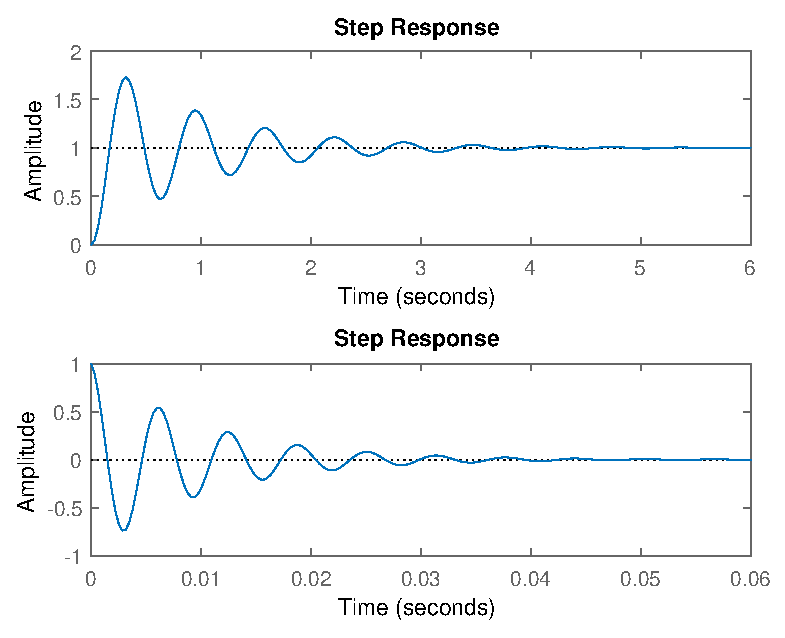
\includegraphics[width=0.6\textwidth]{Imagens/stepResponse.eps}
%	\caption[entrada]{Step response of both low-pass and high-pass modes.}
%	\label{fig:stepResponse}
%\end{figure}

\begin{figure}[!htb]
	\centering
	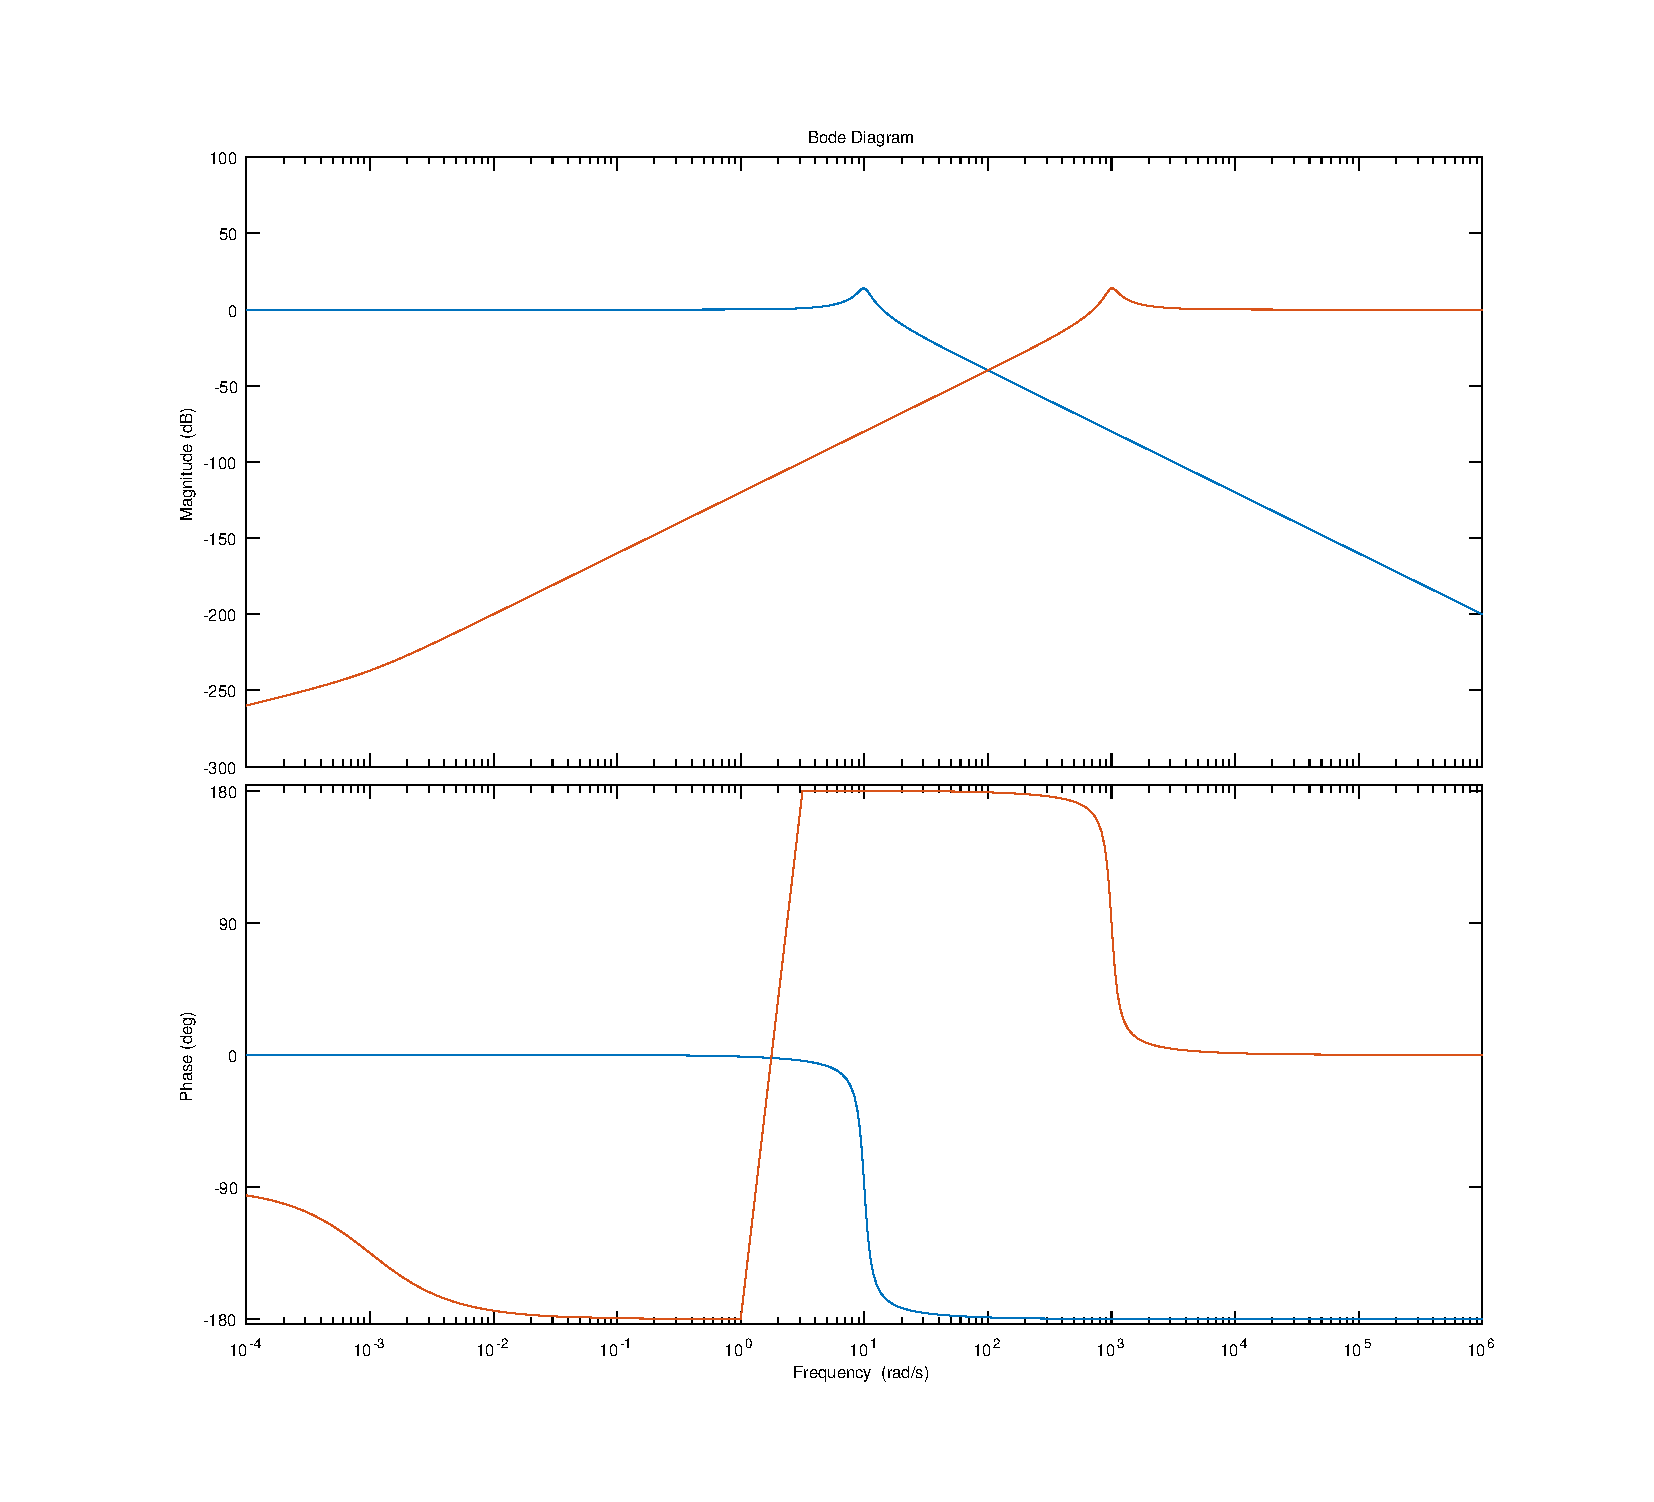
\includegraphics[width=0.6\textwidth]{Imagens/bode.eps}
	\caption[Bode diagram of both modes]{Bode diagram of both modes. Blue represent the low-pass system and red the high-pass system.}
	\label{fig:bode}
\end{figure}

%\begin{figure}[!htb]
%	\centering
%	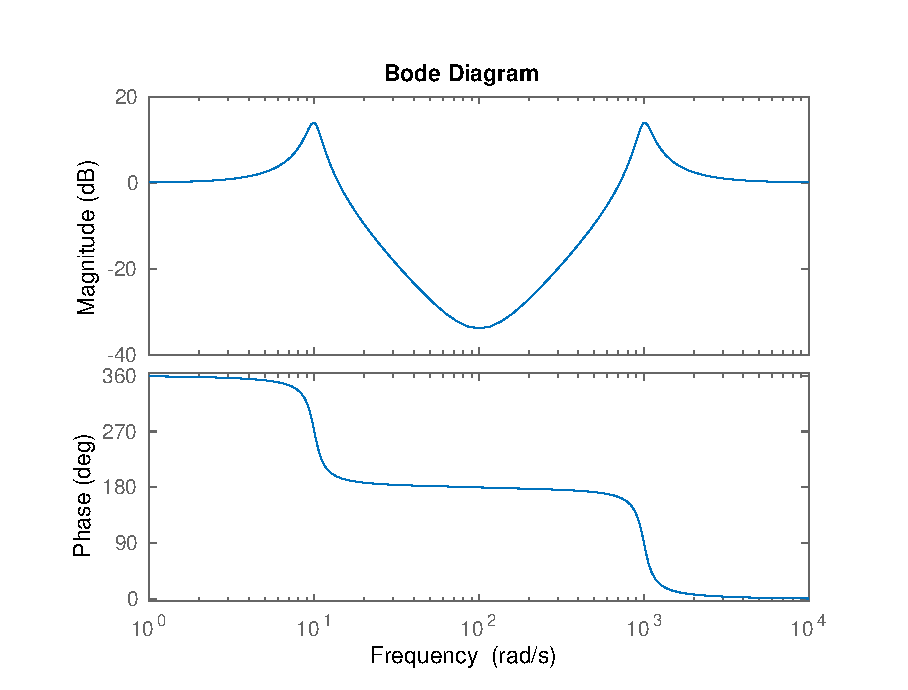
\includegraphics[width=0.6\textwidth]{Imagens/bodeS.eps}
%	\caption[entrada]{Bode diagram of the resulting fourth order system.}
%	\label{fig:bodeS}
%\end{figure}


The resulting fourth order system is described as a state space representation, in a modal canonical form given by:

\begin{align}
\dot{x}(t) & = Ax(t) + Bu(t) \label{eq:sys_beg}\\
y(t) & = Cx(t) + Du(t)
\end{align}


\noindent
where $x(t) \in \mathbf{R}^4$ is the state vector, $u(t) \in \mathbf{R}^1$ is the single input vector and $y(t) \in \mathbf{R}^1$ is the single output vector, and

\begin{align}
A & =\begin{bmatrix}
-100 & 994.99 & 0 & 0\\
-994.99 & -100 & 0 & 0\\
0 & 0 & -1 & 9.949\\
0 & 0 & -9.949 & -1
\end{bmatrix}, \\
B & =\begin{bmatrix}
-24.6435 \\
-18.8943 \\
-4.1746 \\
-0.2675
\end{bmatrix}, \\
C & =\begin{bmatrix}
24.41 & -21.2522 & -0.1537 & 2.3977 \\
\end{bmatrix}, \\
D & =1. \label{eq:sys_end}
\end{align}

%
%\begin{equation}\label{eq:sistemaLinear}
%\begin{split}
%Z_{de} & := (\partial Z/\partial \delta_e)/m = -61.655 \ m/s^2,\\
%Z_q & := (\partial Z/\partial q)/m = -5.132 \ m/s,\\
%Z_w & := (\partial Z/\partial W)/m = -3.1332 \ s^{-1},\\
%M_{de} & := (\partial M/\partial \delta_e)/I_y = -40.465 \ s^{-2},\\
%M_q & := (\partial M/\partial q)/I_y = -2.6864 \ s^{-1},\\
%M_w & := (\partial M/\partial W)/I_y = -0.04688 \ (s-m)^{-1},\\
%\tau & = 0.1 \ s \\
%U_o & = 306.42 \ m/s
%\end{split}
%\end{equation}

We simulate a pseudo-random binary sequence (PRBS) as input, with 200 samples, as shown in Figure~\ref{fig:prbs}.

\begin{figure}[!htb]
	\centering
	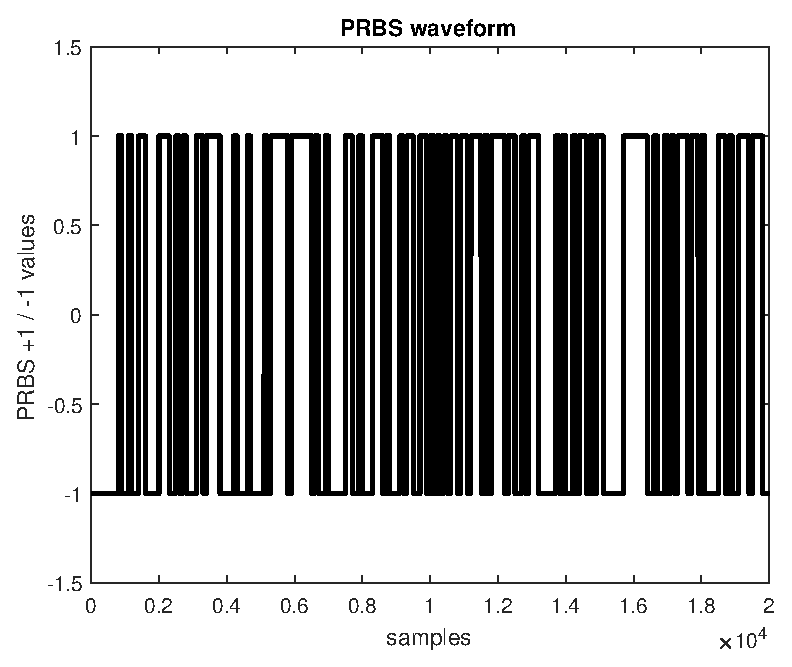
\includegraphics[width=0.8\textwidth]{Imagens/prbs.eps}
	\caption[PRBS samples used as input]{200 PRBS samples used as input}
	\label{fig:prbs}
\end{figure}

The PRBS signal is used as input to the low-pass and high-pass systems separately, considering two different time frames, of 2 and 20 seconds. The results of the four linear simulations are shown in Figure~\ref{fig:sys_results}. We can see a much faster response from the high-pass filter in both cases, as expected.

 \begin{figure}[!htb]
 	\centering
 	\subfigure[]{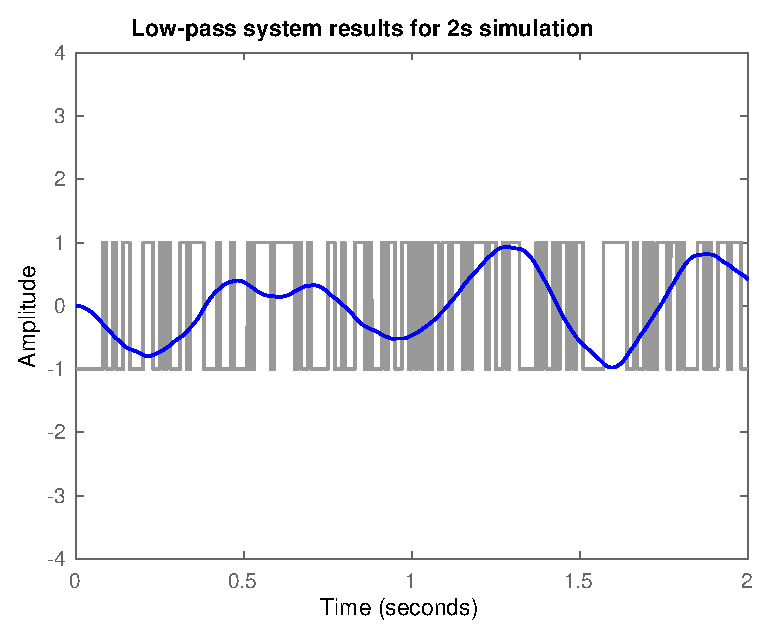
\includegraphics[width=0.49\textwidth]{Imagens/lp2s.eps}} 
 	\subfigure[]{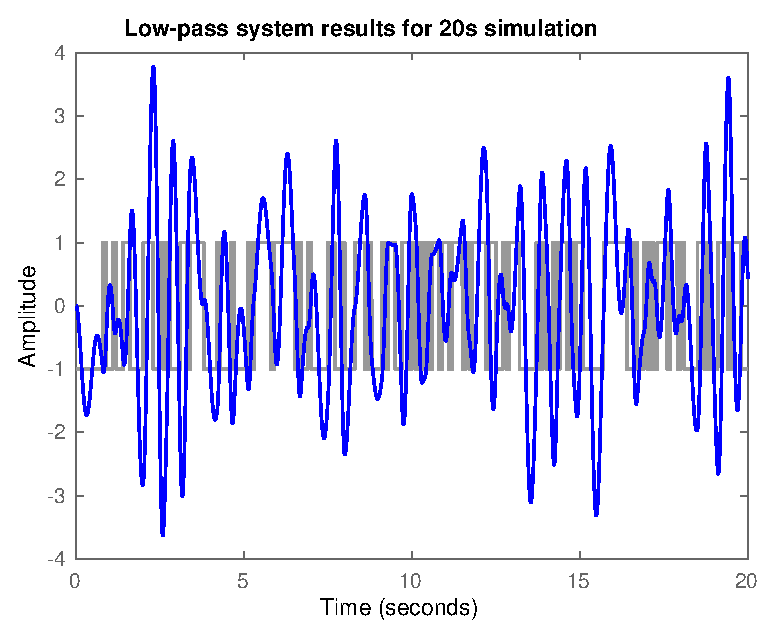
\includegraphics[width=0.49\textwidth]{Imagens/lp20s.eps}}  \\
 	\subfigure[]{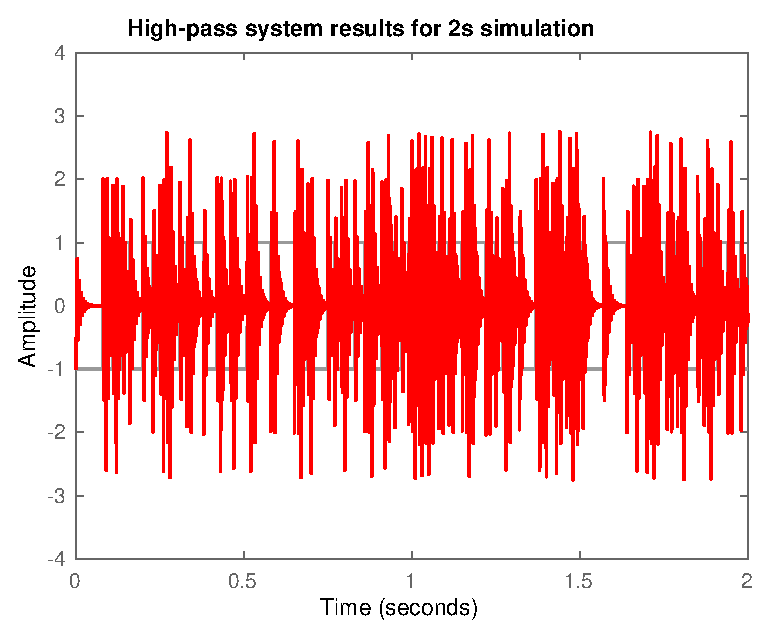
\includegraphics[width=0.49\textwidth]{Imagens/hp2s.eps}}
 	\subfigure[]{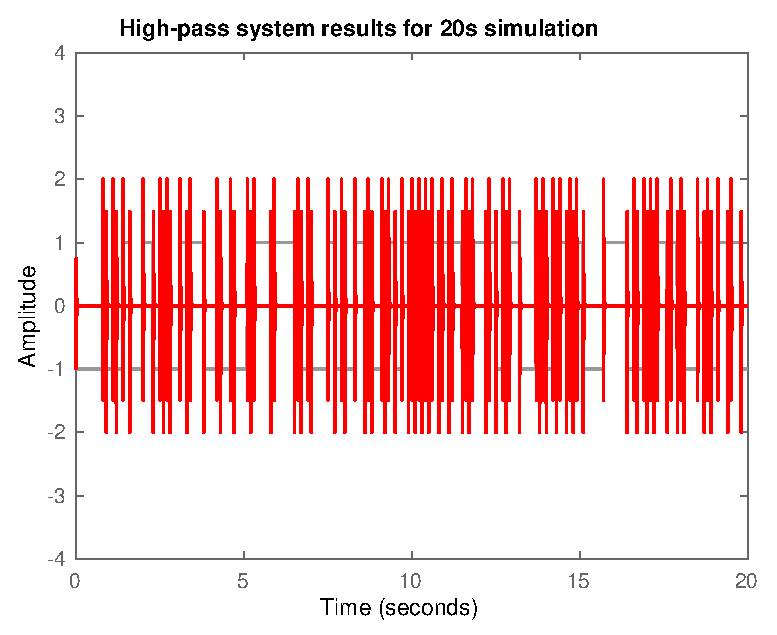
\includegraphics[width=0.49\textwidth]{Imagens/hp20s.eps}}
 	\caption[Linear simulation results for PRBS input in different time frames]{Linear simulation results of the low-pass and high-pass systems separately. Grey lines represent the PRBS input and colored lines the output. Graphs (a) and (b) with blue outputs represent the results of the low-pass system; and (c) and (d) with red outputs, the results of the high-pass system. Graphs on the left show a time frame of 2 seconds of simulations, whereas the ones on the right are the result of a 20 seconds time frame; considering the same 200 samples of PRBS for all four simulations.} 
 	\label{fig:sys_results}
 \end{figure}

The 20 seconds simulation for the high-pass system generates outputs that stabilize very quickly, with a dynamics hard to be observed. Thus, we choose the 2 seconds time frame to simulate the fourth order serialized systems, given by (\ref{eq:sys_beg})-(\ref{eq:sys_end}). The result of the linear simulation of the fourth order system is presented in Figure~\ref{fig:4ordersys2s}.

\begin{figure}[!htb]
	\centering
	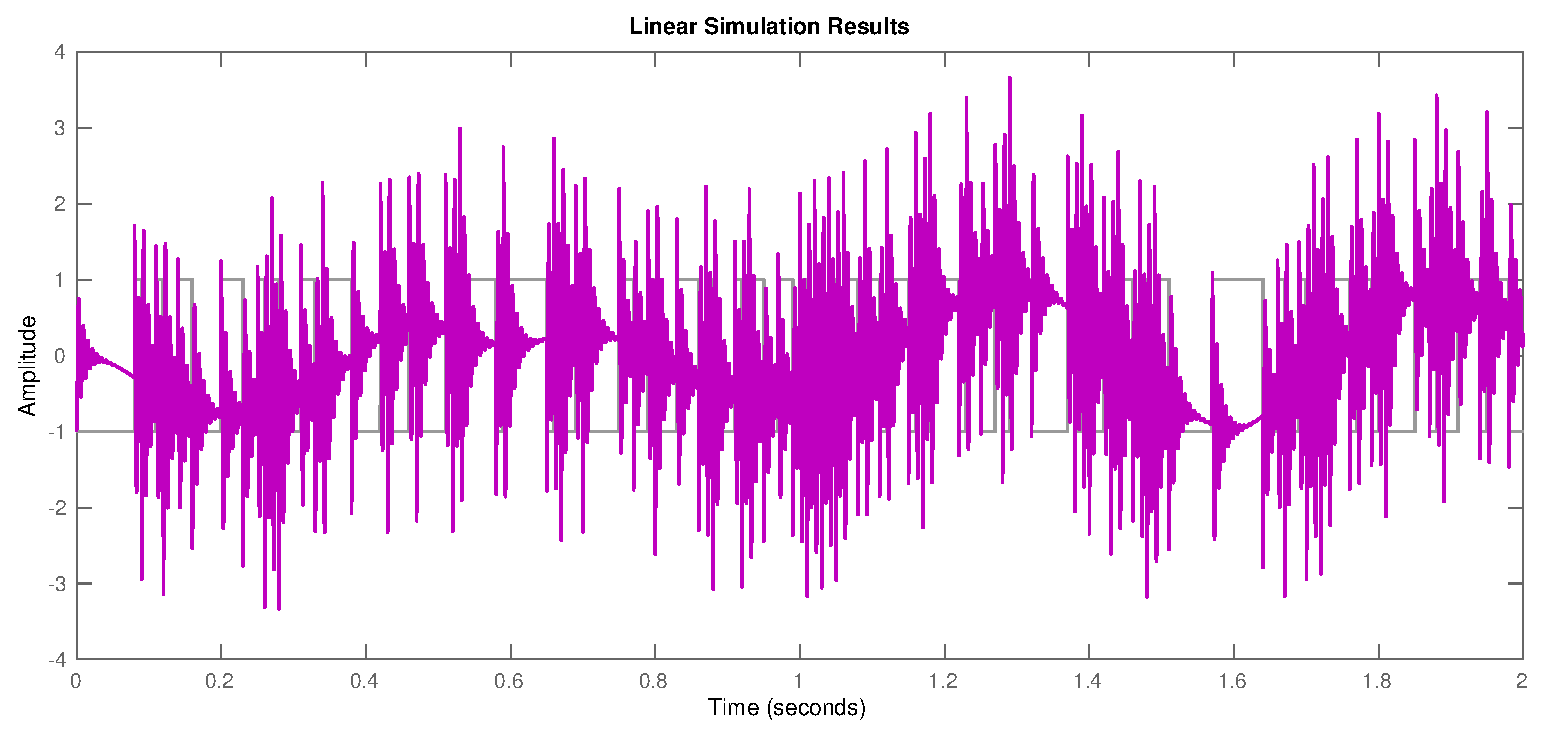
\includegraphics[width=0.8\textwidth]{Imagens/4ordersys2s.eps}
	\caption[Output of the fourth order system to the PRBS input signal]{Output of the fourth order system to the PRBS input signal over a 2 seconds time frame.}
	\label{fig:4ordersys2s}
\end{figure}

System discretization is performed using Matlab\texttrademark's built-in function \texttt{c2d} to produce a discrete-time state space representations according to

\begin{align}
x(t_{k+1}) &= A_{\textrm{d}}(t_k) x(t_k) + B_{\textrm{d}} u(t_k) + w(t_k), \\
y(t_k) &= B_{\textrm{d}}x(t)+D_{\textrm{d}}u(t) + v(t_k)
\end{align}

\noindent
where $\rho(v(t_k)) = \mathcal{N} (0,R)$ and $\rho(w(t_k)) = \mathcal{N} (0,Q)$ are, respectively, the process and observation noise, with zero mean and covariance $R$ and $Q$. When time-stamp is not available, the observation vector is approximated by $\tilde{y}_i \approx y(t_k)$, where $i$ is the index of the next time instant, multiple of $T$. When it is available, discretization is performed using variable time intervals.

\subsection{Linear System Realization}

In this section we present one realization of the state estimation simulation for the system defined by (\ref{eq:sys_beg})-(\ref{eq:sys_end}), the Kalman Filter described in Section~\ref{sec:kalman-filter} and the algorithms modifications explained in Section~\ref{sec:estimation_aperiodic}.  

The parameters are set according to

\begin{align}
\delta t_{\textrm{sim}} &= 10^{-6} \textrm{ s}, \\
T &= 2\times 10^{-3} \textrm{ s}, \\
\lambda &  = 500 \textrm{ Hz}, \\
SNR_{\textrm{obs}} &= 30 \textrm{ dB}, \\
SNR_{\textrm{pro}} &= 30 \textrm{ dB},
\end{align}

\noindent
where $\delta t_{\textrm{sim}}$ is the real system data simulation time-step, $T$ is the regular estimation and input sampling time interval, $\lambda$ is the parameter of Poisson process that describes time instants sequence $t_k, \ \forall k\in \mathbb{N}$ and $SNR_{\textrm{obs}}$ and $SNR_{\textrm{obs}}$ are the signal-to-noise ratio of the observation and process models, respectively. Noise is generated using the \texttt{awgn} function from Matlab\texttrademark. For this realization, it resulted in a measurement noise variance of $R=9.596\times 10^{-4}$ and process noise variance of $Q=9.986\times 10^{-4}$. These exact values were used in the Kalman filter implementation and the estimation results for states $x_1$ and $x_4$ of the algorithms with and without timestamp, in comparison to the true state values are shown in Figures~\ref{fig:StatesWithAndWithoutTimeStamp}.

\begin{figure}[!htb]
	\centering
	\subfigure{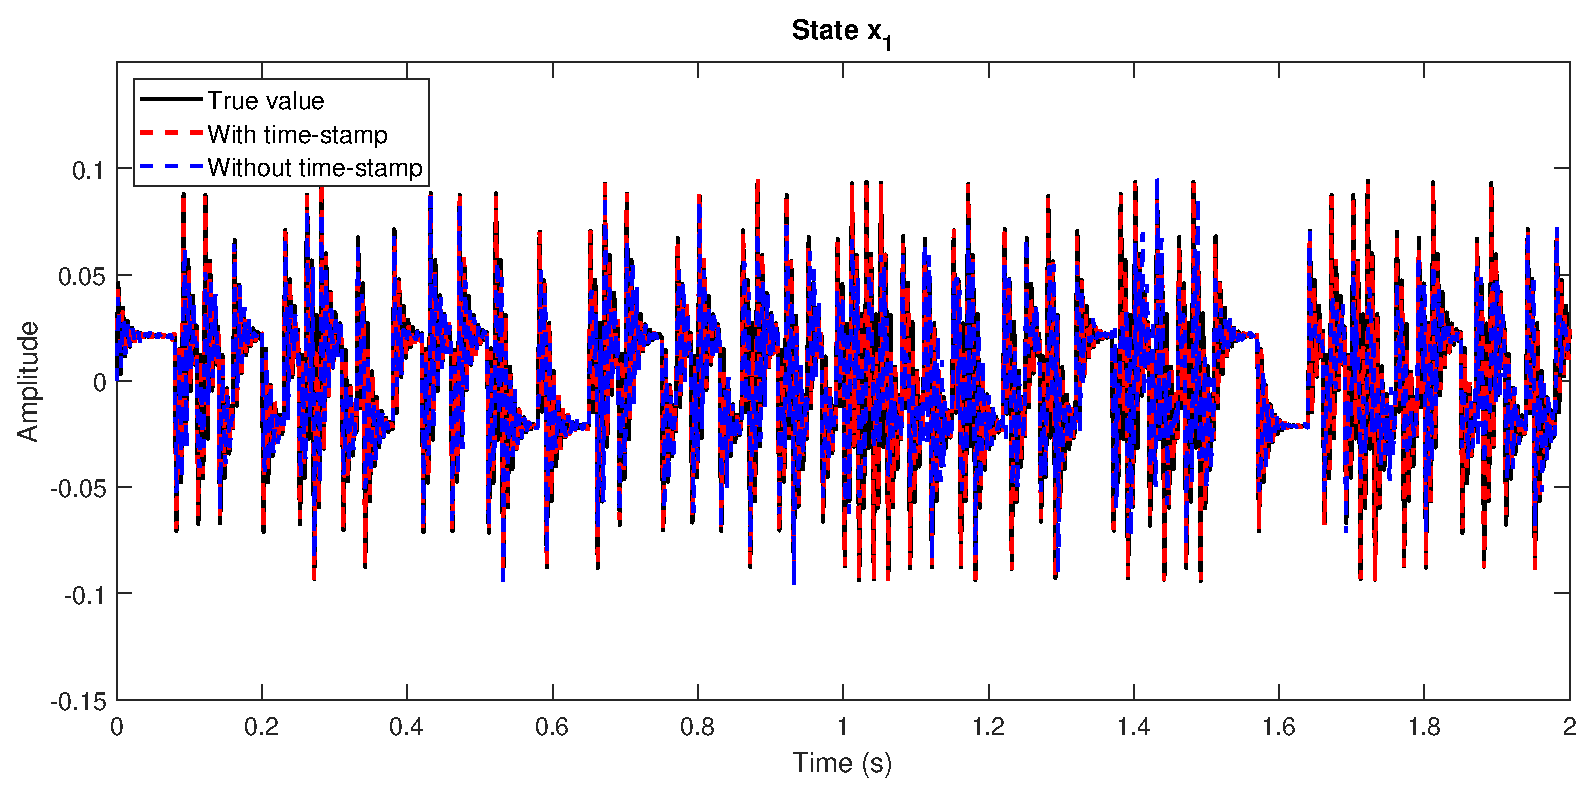
\includegraphics[width=0.8\textwidth]{Imagens/StatesWithTimeStamp.eps}} \\
	\subfigure{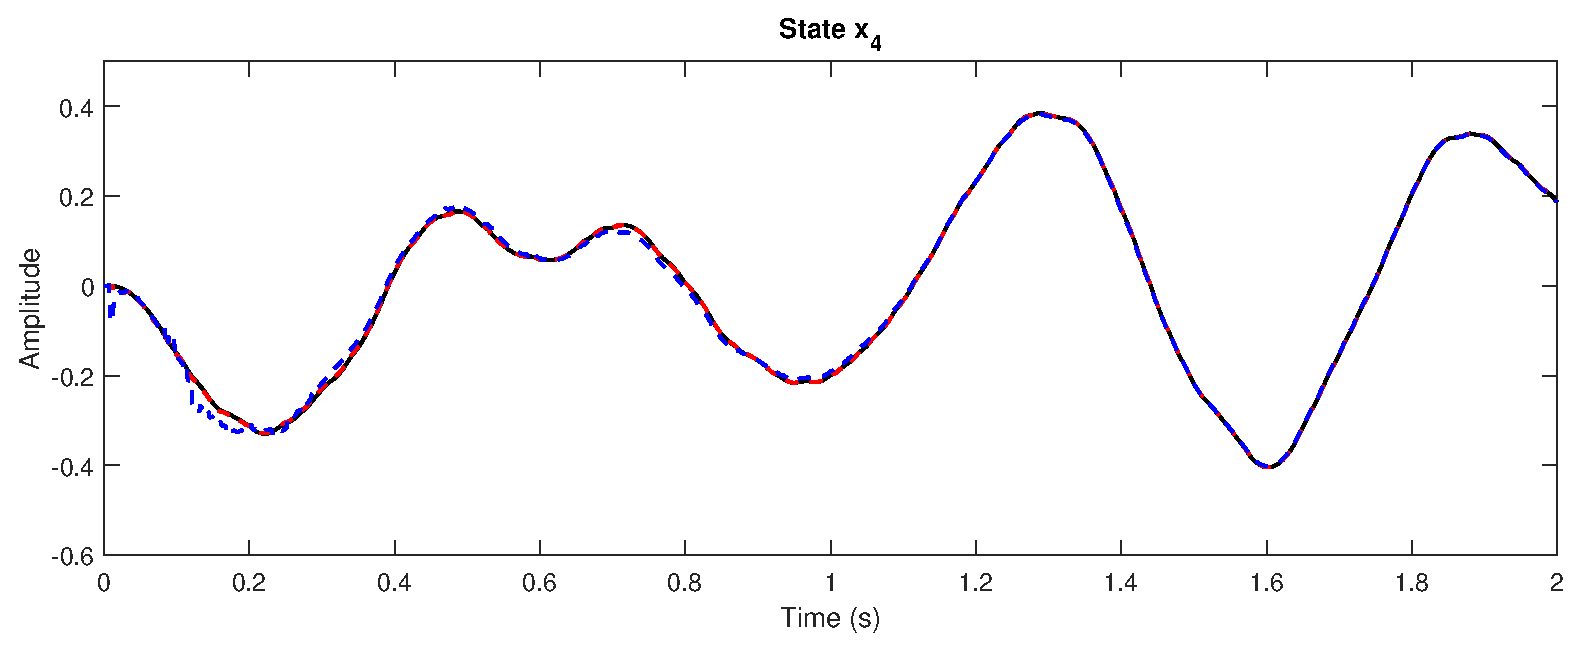
\includegraphics[width=0.8\textwidth]{Imagens/StatesWithoutTimeStamp.eps}}  
	\caption[Estimated and true states]{States $x_1$ and $x_4$ estimates with time-stamp (\textcolor{red}{- -}), without time-stamp (\textcolor{blue}{- -}) and true values (\textcolor{black}{---}).}
	\label{fig:StatesWithAndWithoutTimeStamp}
\end{figure}

For the high-pass system state $x_1$, it is hard to note a significant difference in the estimation performance. However, for state $x_4$, from the low-pass system, the degradation is visible for the algorithm that does not acknowledge time instants $t_k$ information in the estimation process.


Figure~\ref{fig:LinearJevolution} presents a window data from 0 to 0.013 seconds of state $x_2$ RMSE for the algorithms with and without time-stamp. As expected, we observe a distancing from the RMSE at the instant the first observation was taken $t_1$, favoring the algorithm that considers time-stamp. For the time period without observations, the algorithms' RMSE evolve in a similar way. When measurements start to appear back again, we can notice further degradation in the performance when time-stamps are not considered.

\begin{figure}[!htb]
	\centering
	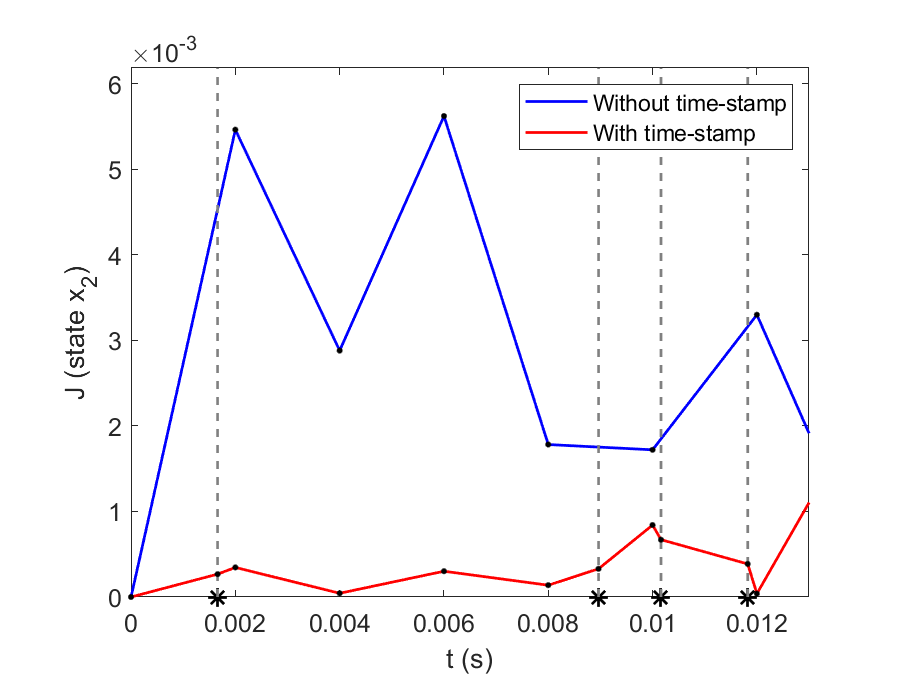
\includegraphics[width=0.8\textwidth]{Imagens/LinearJEvolution.eps}
	\caption[Performance index temporal cut for one realization]{Temporal cut from 0 to 0.013 seconds, for a realization of state $x_2$ RMSE of both estimators, with (\textcolor{red}{---}) and without (\textcolor{blue}{---}) time-stamp. Vertical dashed lines match the measurement sampling instants $t_k$. Black dots represent the estimation instants.}
	\label{fig:LinearJevolution}
\end{figure}

Finally, for this realization, we also present in Figure~\ref{fig:linearConsistency} the single-run consistency tests NEES and NIS as defined in Section~\ref{sec:metrics}. In each graph, the acceptance intervals is marked by horizontal lines. The upper plots (a) and (b) represent the NEES and NIS values, respectively, for the algorithm that considers time-stamp in the estimation process. We can see that the estimates are quite consistent, with the values inside the acceptance region most of the time. In fact, the null hypothesis rejection rate, that is the proportion of times the values were out of their acceptance region, was $0.04$ for NEES, and $0.055$ for NIS, very close the the $0.05$ expected. When time-stamp information was not available, consistency was heavily degraded, with rejection rates escalated to $0.61$ and $0.43$, respectively. Moreover, NEES and NIS values were so high in some occasions, that the acceptance region is hardly visible in the graphs. In practice, such a consistency degradation means that estimation covariances are highly underestimated.

 \begin{figure}[!htb]
	\centering
	\subfigure[]{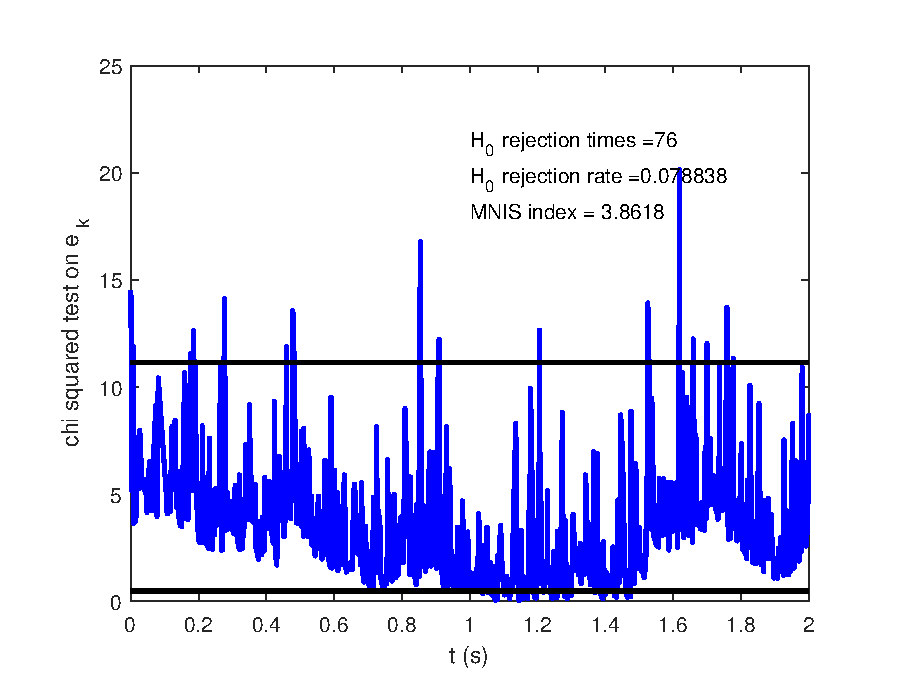
\includegraphics[width=0.49\textwidth]{Imagens/chi_e_with.eps}} 
	\subfigure[]{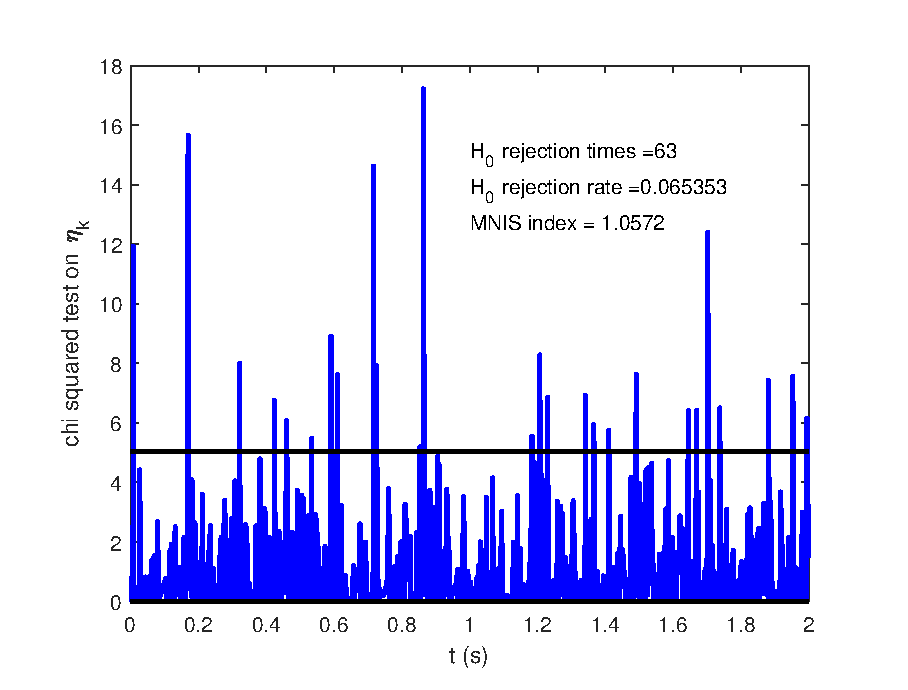
\includegraphics[width=0.49\textwidth]{Imagens/chi_eta_with.eps}}  \\
	\subfigure[]{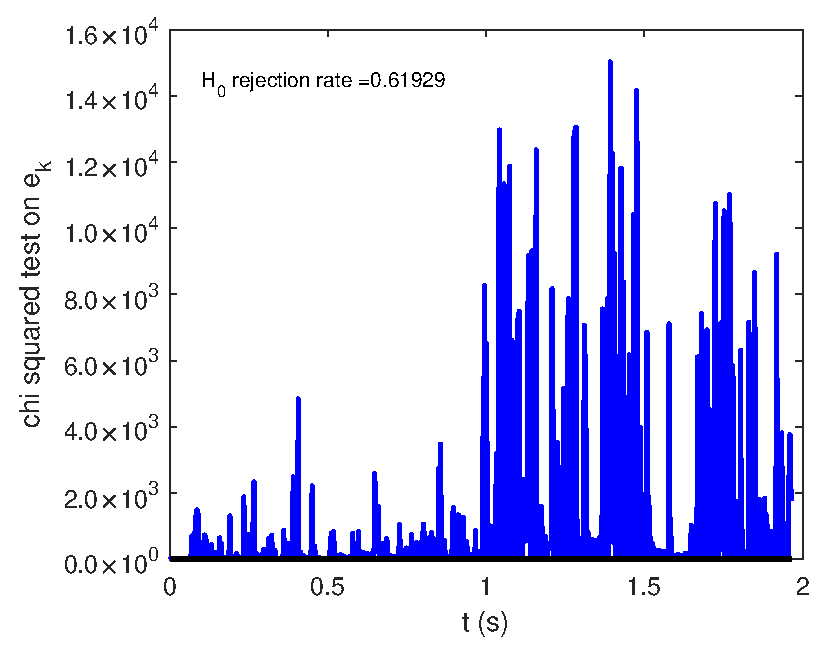
\includegraphics[width=0.49\textwidth]{Imagens/chi_e_without.eps}}
	\subfigure[]{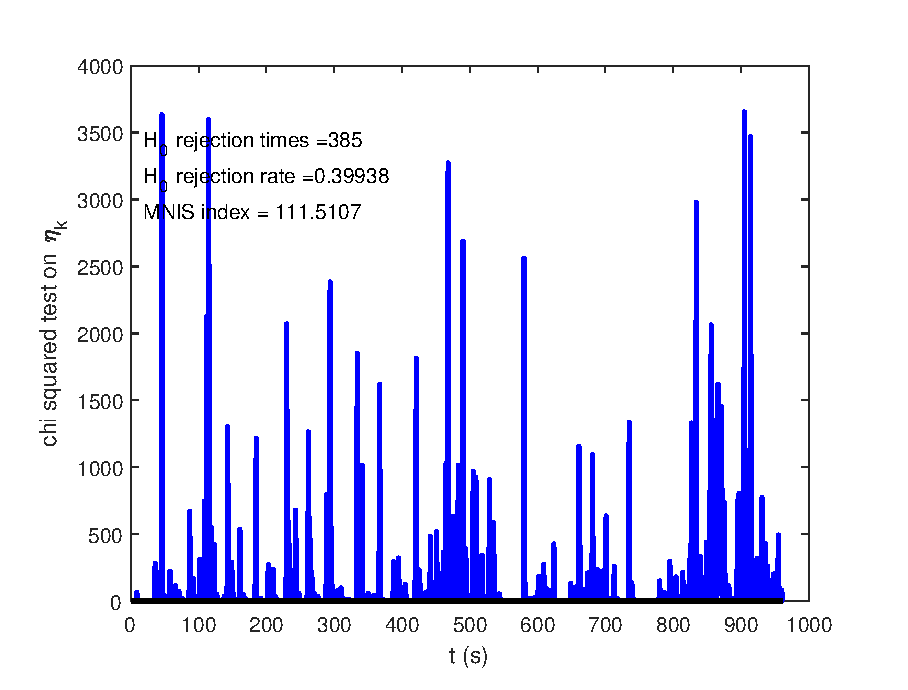
\includegraphics[width=0.49\textwidth]{Imagens/chi_eta_without.eps}}
	\caption[Consistency tests for linear system]{Consistency tests NEEs and NIS for the linear system state estimation with time-stamps (a) and (b); and without time-stamp (c) and (d). Horizontal lines define the acceptance region upper and lower limits, for a significance level $\alpha=0.05$. In each graph, the null hypothesis $H_0$ rejection rate is also presented.}
	\label{fig:linearConsistency}
\end{figure}

In the next sections we study the scenarios described in Section~\ref{sec:scenarios}. Only one state per mode is evaluated, namely $x_1$ and $x_4$, for simplicity.

\subsection{Measurement Signal-to-Noise Ratio Variation}\label{sec:ruido-AC}

For the first simulation scenario, we consider SNR variation of $60$, $50$, $40$, $20$, and $10$, $\textrm{dB}$ both for the process and observation models. Regular estimation time interval $T$ is maintained fixed at $T=0.002 \textrm{s}$  and $\alpha=1$, thus $\lambda=500 \textrm{Hz}$. For a 100-run simulation, obtained results for accuracy and consistency are presented in Figure~\ref{fig:linearNoise} with the corresponding $95\%$ confidence intervals.


 \begin{figure}[!htb]
	\centering
	\subfigure[]{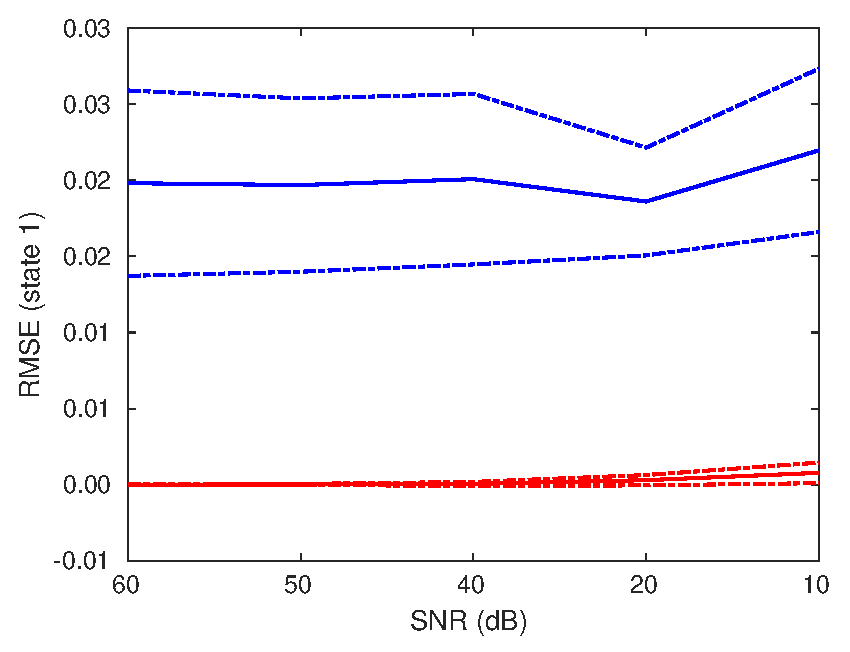
\includegraphics[width=0.49\textwidth]{Imagens/linearNoise_x1_rmse.eps}} 
	\subfigure[]{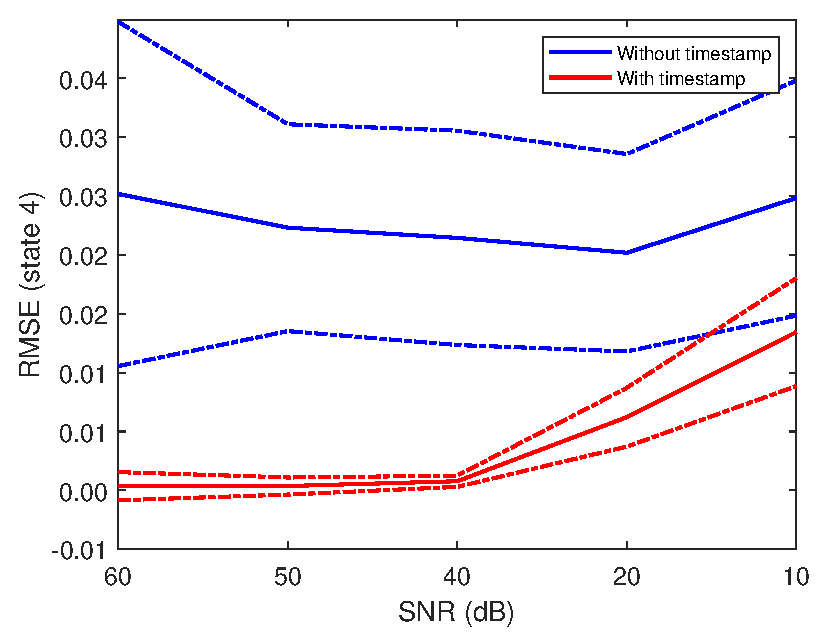
\includegraphics[width=0.49\textwidth]{Imagens/linearNoise_x4_rmse.eps}}  \\
	\subfigure[]{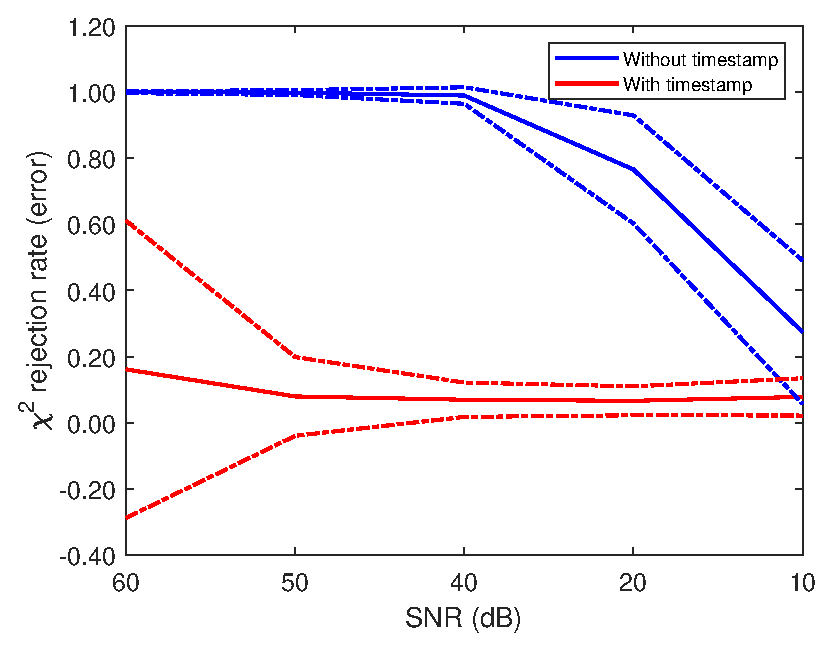
\includegraphics[width=0.49\textwidth]{Imagens/linearNoise_NEES.eps}}
	\subfigure[]{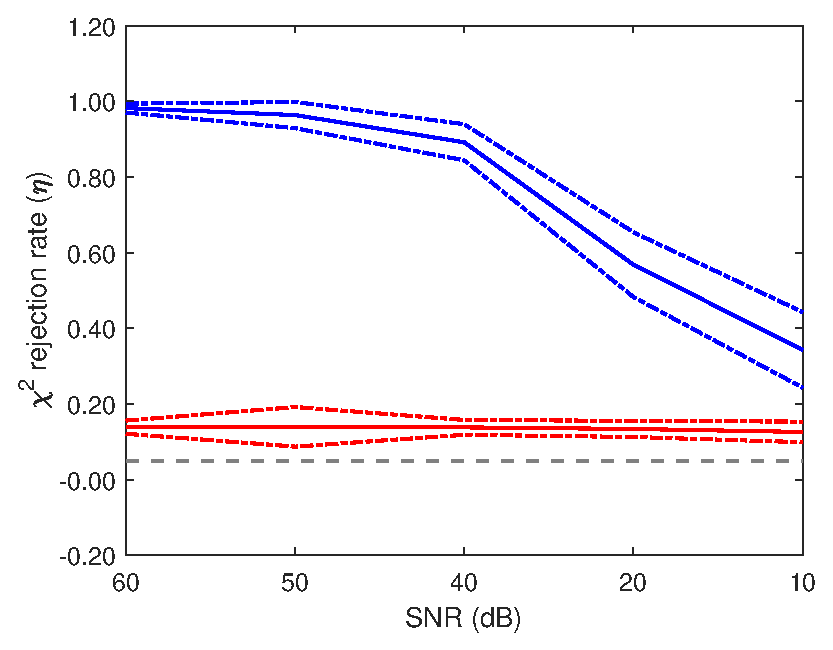
\includegraphics[width=0.49\textwidth]{Imagens/linearNoise_NIS.eps}}
	\caption[Linear system estimation performance, as a function of input and observation SNR]{Linear system estimation performance indexes with $95\%$ confidence intervals, as a function of input and observation SNR, for algorithms with (\textcolor{red}{---}) and without (\textcolor{blue}{---}) time-stamp. Accuracy values for states $x_1$ and $x_2$ are shown in (a) and (b), respectively. Consistency results are in (c) and (d) for NEES and NIS tests, respectively.}
	\label{fig:linearNoise}
\end{figure}

Results suggest that for higher SNR levels, that is less noise present in data, taking into account time-stamp information plays an important role, both for accuracy and consistency. When noise levels increase, indexes approximate for both algorithms. Consistency tests for the algorithm with time-stamp remains almost constant for all SNR values, whereas for the algorithm without time-stamp they decrease to values that do not differ statistically from both methods.


%\subsubsection{Changing only measurement noise}
%
%\begin{figure}[!htb]
%	\centering
%	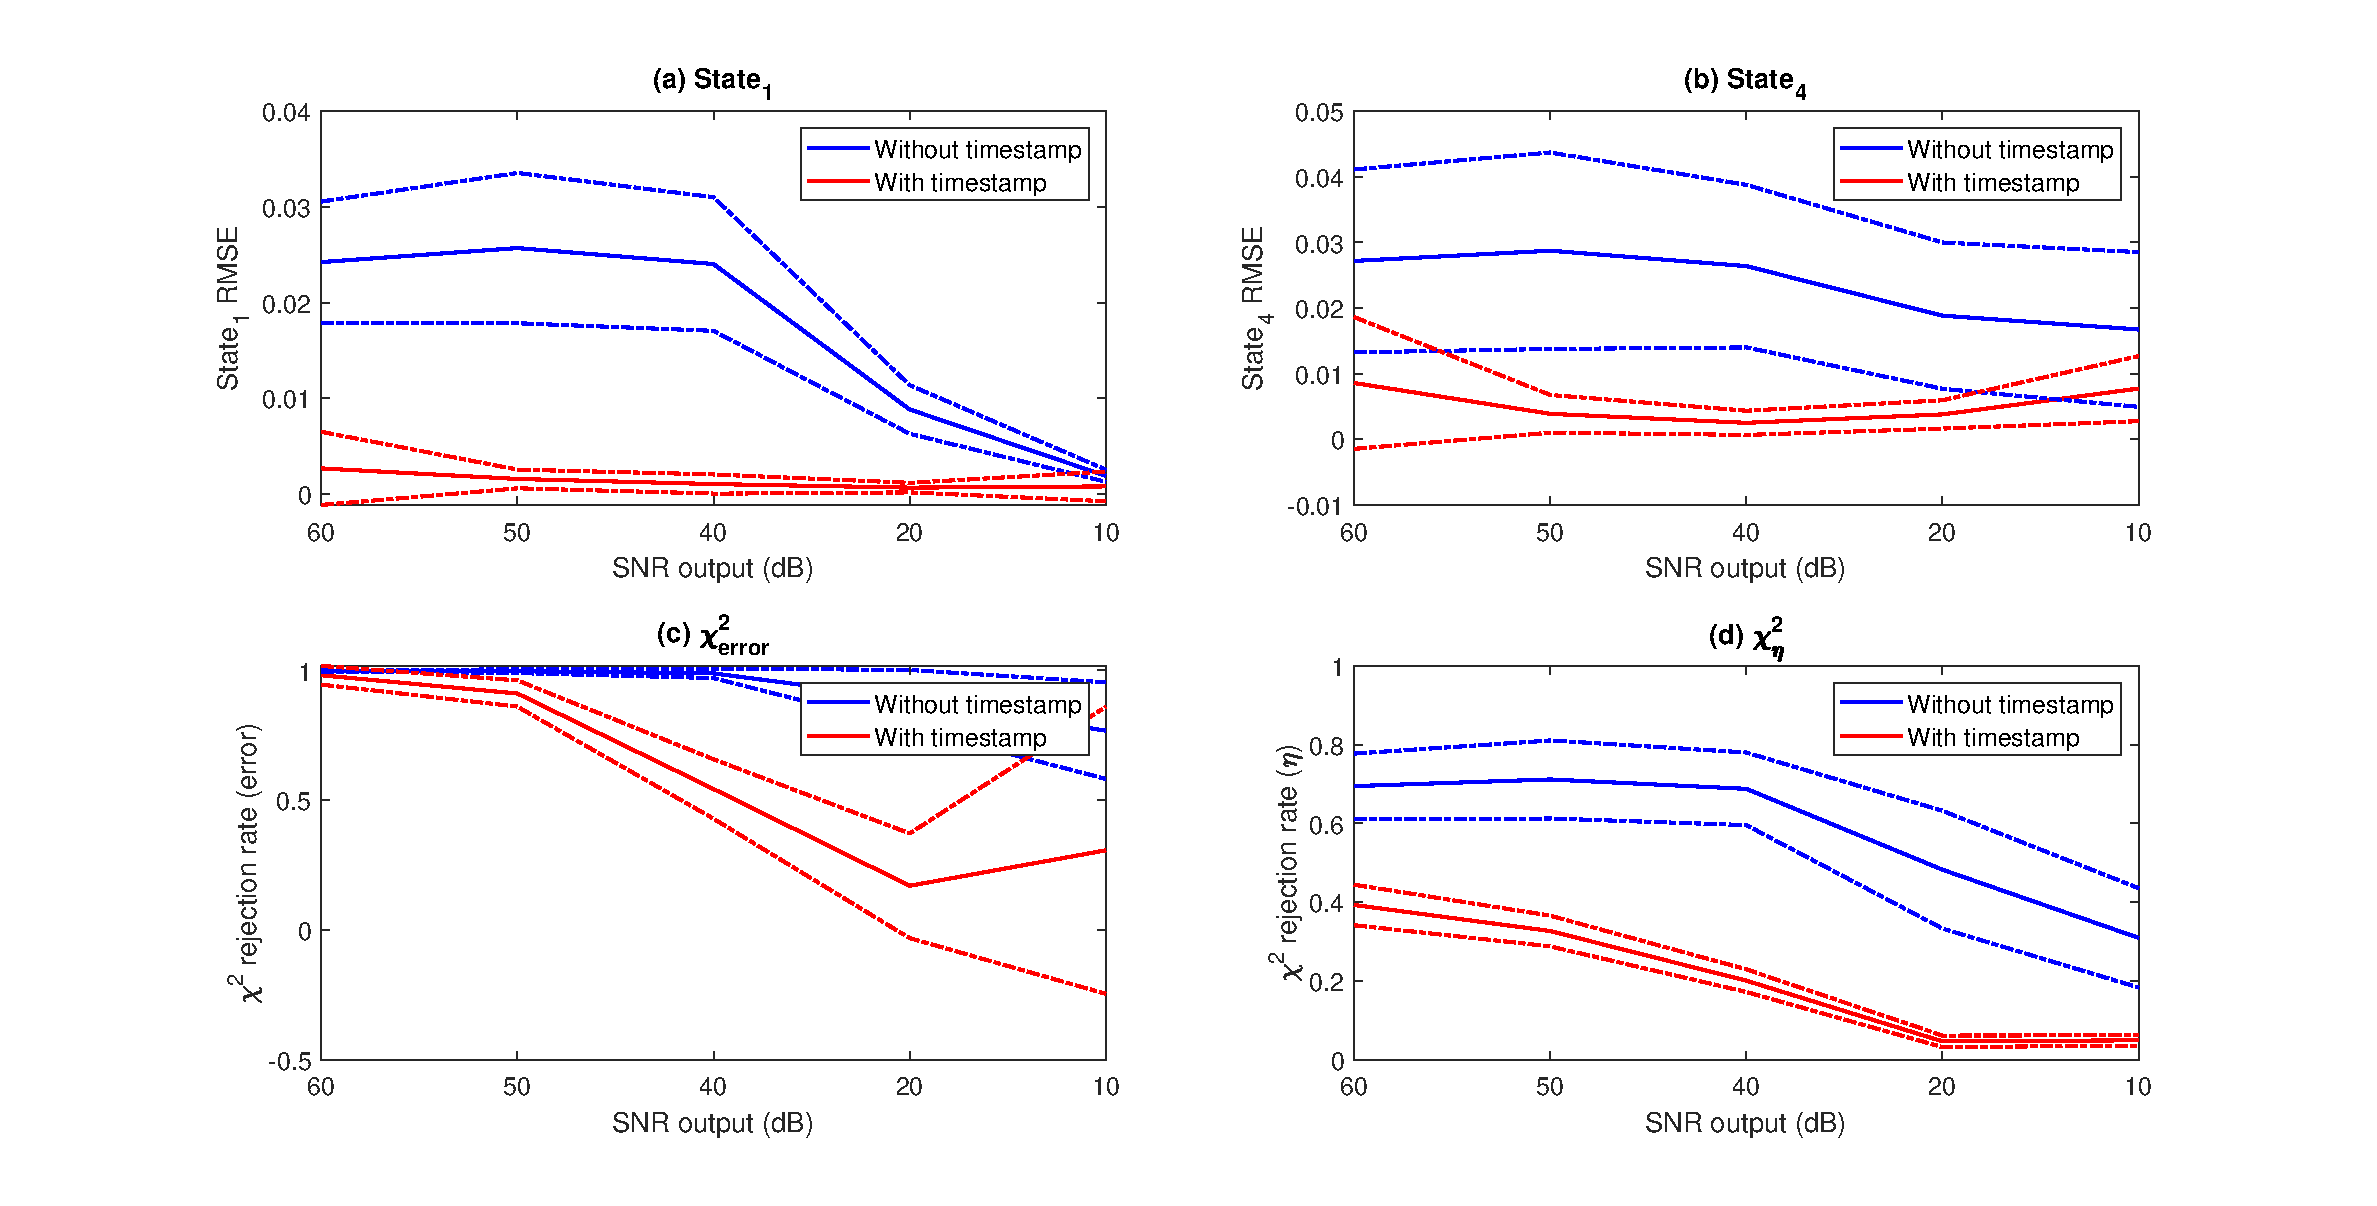
\includegraphics[width=1\textwidth]{Imagens/noise_results_all.eps}
%	\caption[Performance, as a function of observation SNR]{Performance, as a function of observation SNR.}
%	\label{fig:ulinearSamp2}
%\end{figure} 
%
%
%
%%	
%%\begin{figure}[H]
%%	\centering
%%	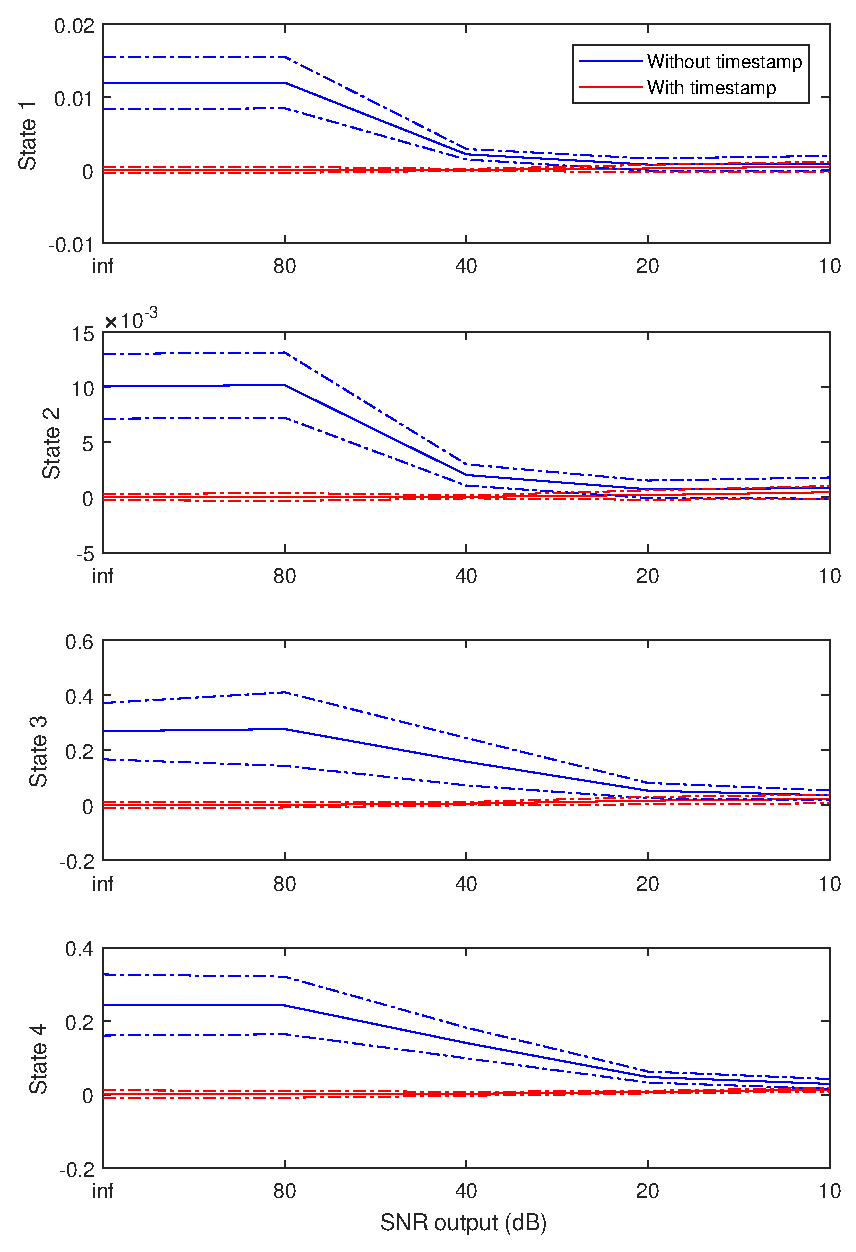
\includegraphics[width=0.8\textwidth]{Imagens/linearNoise.eps}
%%	\caption[entrada]{Root mean square error variation, as a function of measurement noise for both KF algorithms, considering and not considering time-stamp}
%%	\label{fig:linearNoise}
%%\end{figure} 


\subsection{Average Sampling Rate Variation}\label{sec:lambda-AC}

In the second simulation scenario for the linear system, we consider an average sampling rates of observation variation of $\lambda \ =\ 0.001,\ 0.002,\ 0.05,\ \textrm{and } 0.1 \textrm{ Hz}$. Relation between $\lambda$ and $T$ is kept constant $\alpha=1$. SNR levels for process and observation models are chosen to be $SNR_{\textrm{obs}} = SNR_{\textrm{pro}} = 30 \ \textrm{dB}$. Simulation was carried out 100 times and performance indexes for accuracy and consistency are shown in Figure~\ref{fig:linearSamp} with corresponding $95\%$ confidence intervals. 

 \begin{figure}[!htb]
	\centering
	\subfigure[]{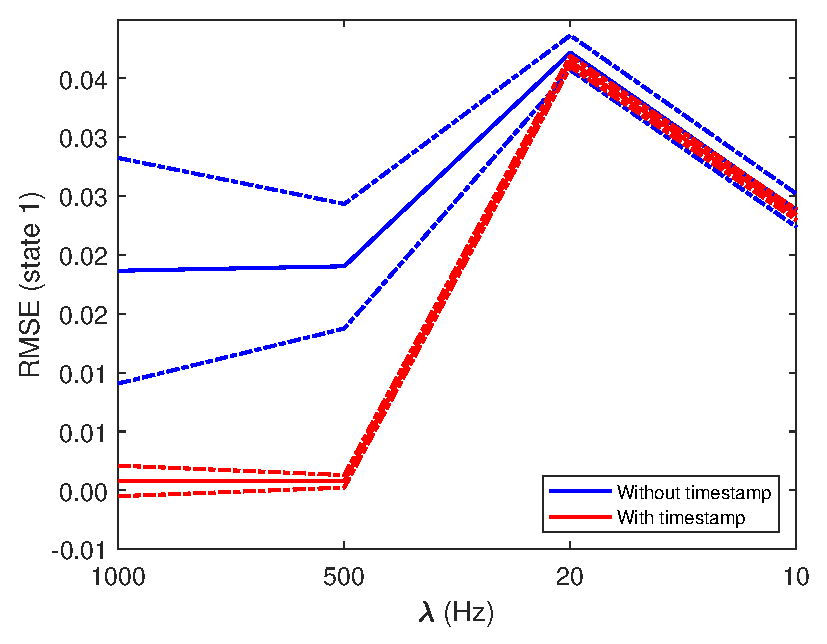
\includegraphics[width=0.49\textwidth]{Imagens/linearSamp_x1_rmse.eps}} 
	\subfigure[]{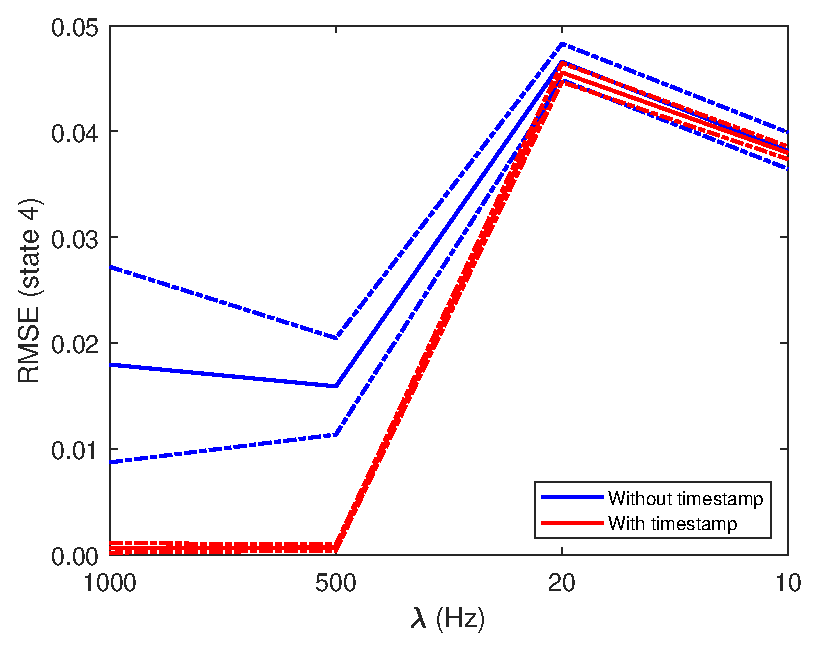
\includegraphics[width=0.49\textwidth]{Imagens/linearSamp_x4_rmse.eps}}  \\
	\subfigure[]{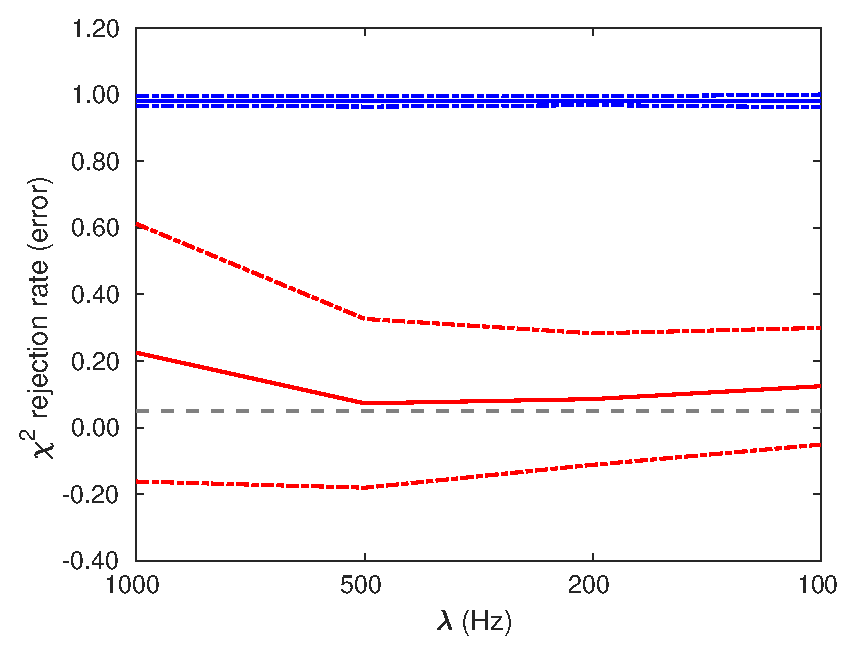
\includegraphics[width=0.49\textwidth]{Imagens/linearSamp_NEES.eps}}
	\subfigure[]{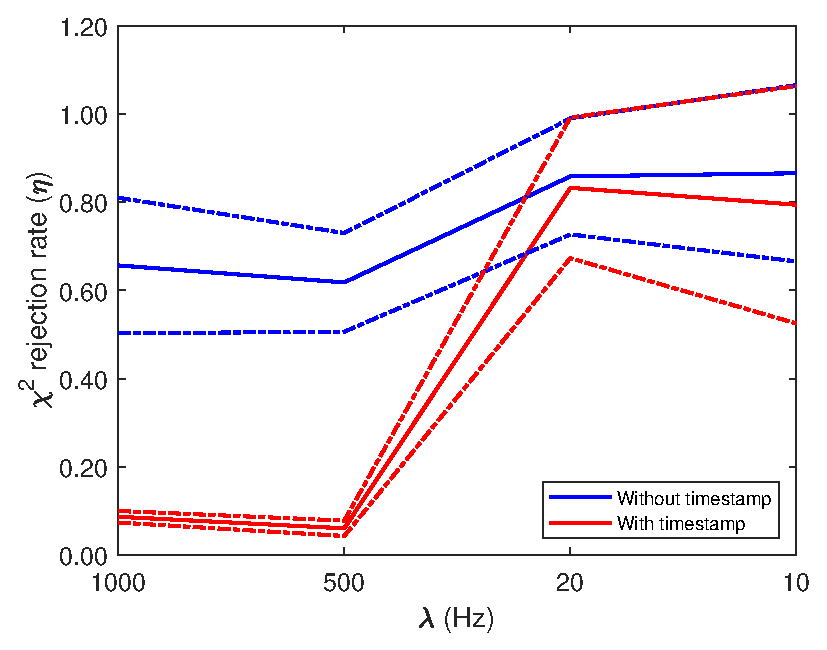
\includegraphics[width=0.49\textwidth]{Imagens/linearSamp_NIS.eps}}
	\caption[Linear system estimation performance, as a function of input and observation SNR]{Linear system estimation performance indexes with $95\%$ confidence intervals, as a function of average time interval $\lambda^{-1}$, for algorithms with (\textcolor{red}{---}) and without (\textcolor{blue}{---}) time-stamp. Accuracy values for states $x_1$ and $x_2$ are shown in (a) and (b), respectively. Consistency results are in (c) and (d) for NEES and NIS tests, respectively.}
	\label{fig:linearSamp}
\end{figure}

In this case, the smaller the $\lambda$ the higher is the difference in algorithm performances, in favor of the one that considers time-stamp information. The high values used for simulation caused both algorithms to perform with no statistically significant difference. It suggests that, the more spaced time intervals of observations, the bigger is the importance of incorporating time instant information in the estimation process. That can be explained by the fact that in such cases, the approximation error of $t_k$ is higher and so is the additional noise introduced by data assimilation performed at incorrect time instants.


\subsection{Regular and Average Irregular Time Interval Relation Variation}\label{sec:alpha-AC}

The last linear system case study is simulated considering a variation of $\alpha = \ 5,\ 3,\ 2,\ \textrm{and } 1$. Other parameters are kept constant, namely $\lambda=500 \textrm{ Hz}$, and $SNR_{\textrm{obs}} = SNR_{\textrm{pro}} = 30 \ \textrm{dB}$. Once again, a 100-run simulation is performed and results are shown in Figure~\ref{fig:linearAlpha}.


 \begin{figure}[!htb]
	\centering
	\subfigure[]{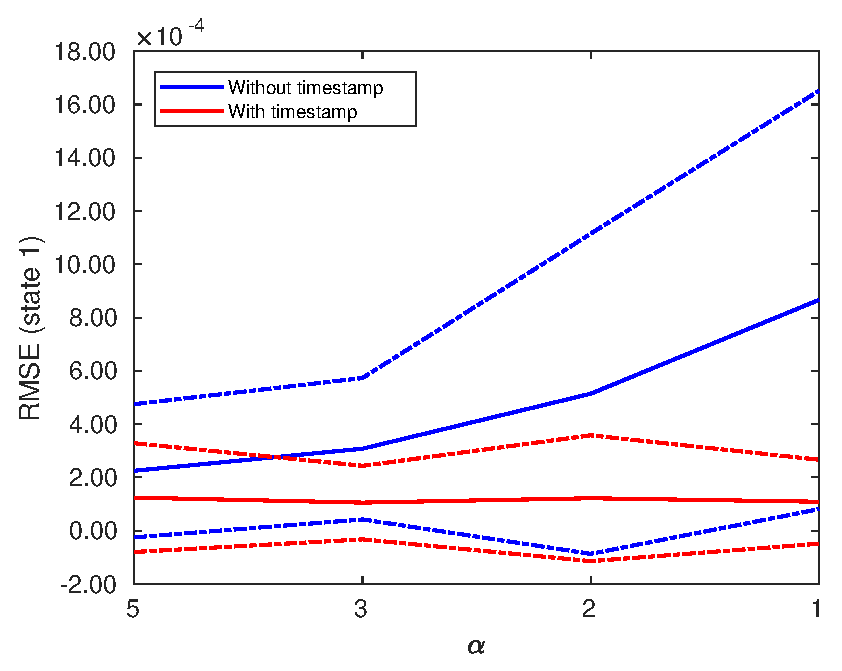
\includegraphics[width=0.49\textwidth]{Imagens/linearAlpha_x1_rmse.eps}} 
	\subfigure[]{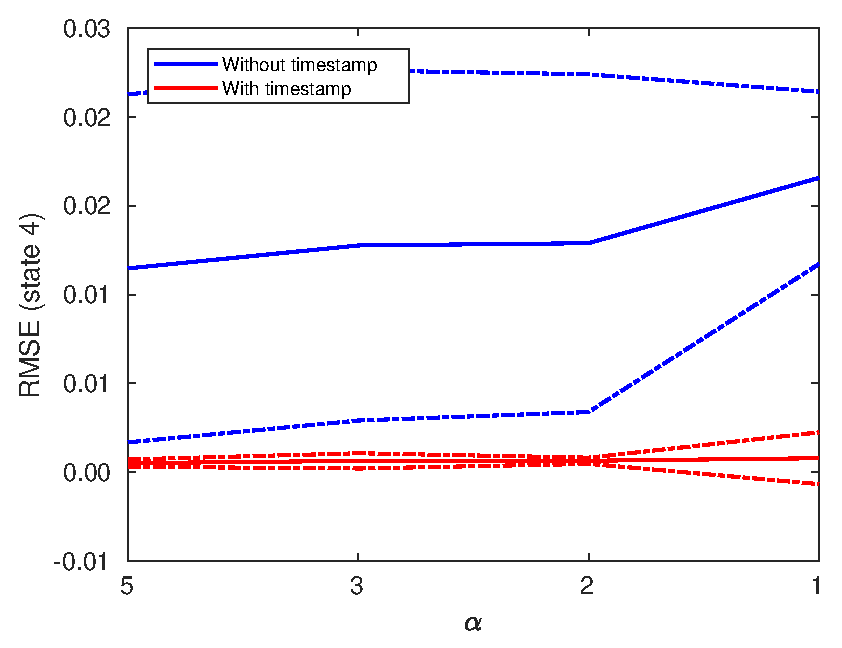
\includegraphics[width=0.49\textwidth]{Imagens/linearAlpha_x4_rmse.eps}}  \\
	\subfigure[]{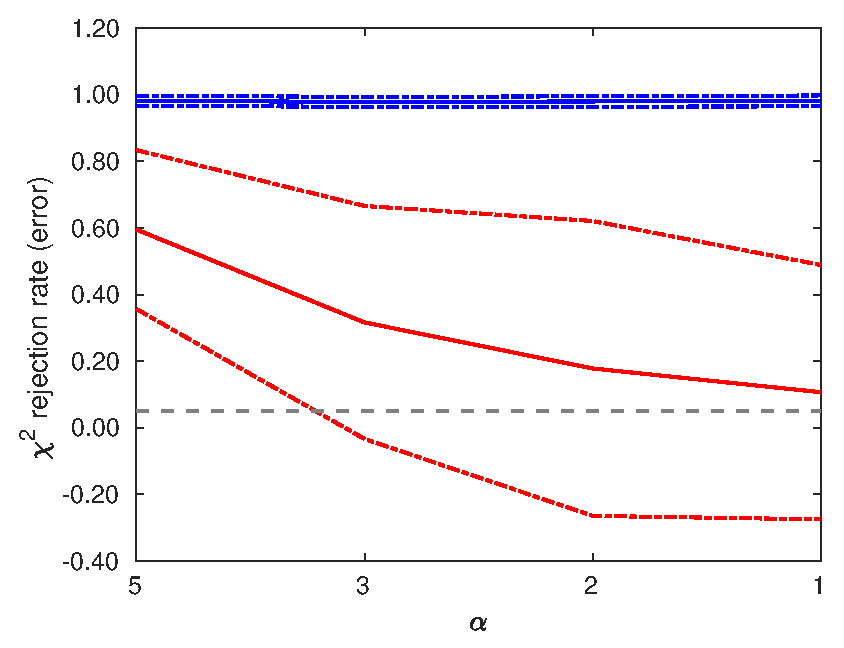
\includegraphics[width=0.49\textwidth]{Imagens/linearAlpha_NEES.eps}}
	\subfigure[]{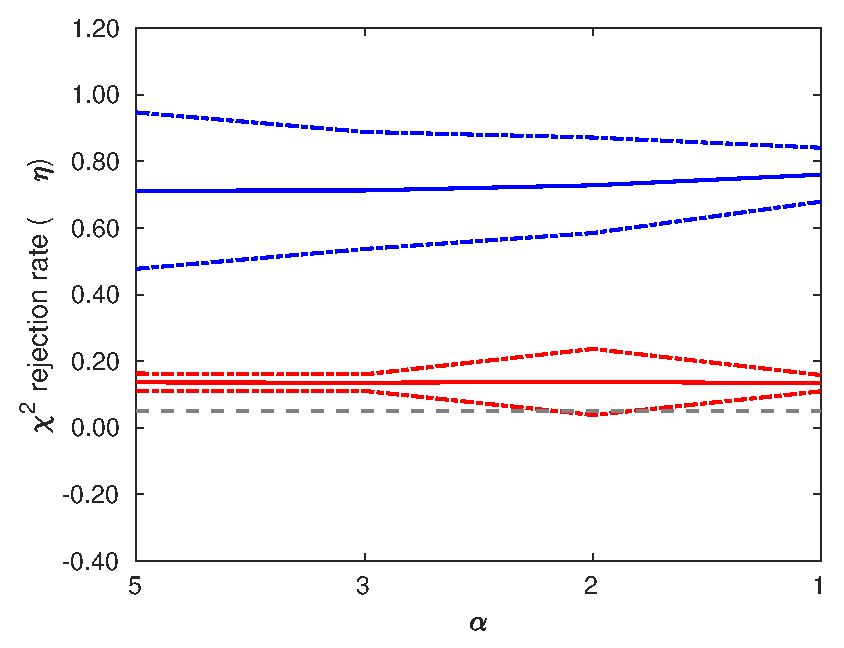
\includegraphics[width=0.49\textwidth]{Imagens/linearAlpha_NIS.eps}}
	\caption[Linear system estimation performance, as a function of input and observation SNR]{Linear system estimation performance indexes with $95\%$ confidence intervals, as a function of $\alpha$, for algorithms with (\textcolor{red}{---}) and without (\textcolor{blue}{---}) time-stamp. Accuracy values for states $x_1$ and $x_2$ are shown in (a) and (b), respectively. Consistency results are in (c) and (d) for NEES and NIS tests, respectively.}
	\label{fig:linearAlpha}
\end{figure}


In this case, performance remained almost constant both for accuracy and consistency, when time-stamp information was available, suggesting that it does not depend on $\alpha$ values. On the other hand, results for the algorithm that does not consider time-stamp are better when regular estimation sampling rate is higher. That is, when input information is available at faster rates than the average sampling rate of observations, knowing the exact time instant $t_k$ becomes less important.

%
%\subsection{Average Time Delay}\label{sec:dt-AC}
%
%\todo[inline,caption={Falta variar o atraso nas medi��es}]{Ainda ter� uma se��o com a varia��o do time-delay e seu impacto no desempenho}


\section{Unicycle Position Estimation}

\todo[inline]{Falta incluir os resultados dos testes NEES e NIS}

We now consider a non-linear system given by a nonholomonic moving robot, which position in the $xy$-plane we want to estimate. In many real target tracking problems such as this, measurements are available by unsynchronized cameras through an internet network, for instance. Or multiple GPS sensors might be used in a centralized architecture without data alignment and association. These configurations are keen to sampling irregularities, which motivates our choice.

\subsection{System Description}

Consider a nonholomonic moving robot, with the cinematic process model given by

\setlength{\abovedisplayskip}{0.5pt}

\begin{equation}\label{eq:sistema}
\begin{split}
\dot{p}_\textrm{x} & = v\cos (\theta),\\
\dot{p}_\textrm{y} & = v\sin (\theta),\\
\dot{\theta}  & = u_1(t),\\
\dot{v} & = u_2(t),
\end{split}
\end{equation}

\noindent
where $p_\textrm{x}$ and $p_\textrm{y}$ are the position coordinates, $\theta$ the angular orientation, $v$ the linear velocity and inputs $u_1$ and $u_2$ are the angular velocity $\omega$ and the linear acceleration $a$, respectively. Figure~\ref{fig:robot} shows a schematic of the robot and its states,

\begin{figure}[!htb]
	\centering
	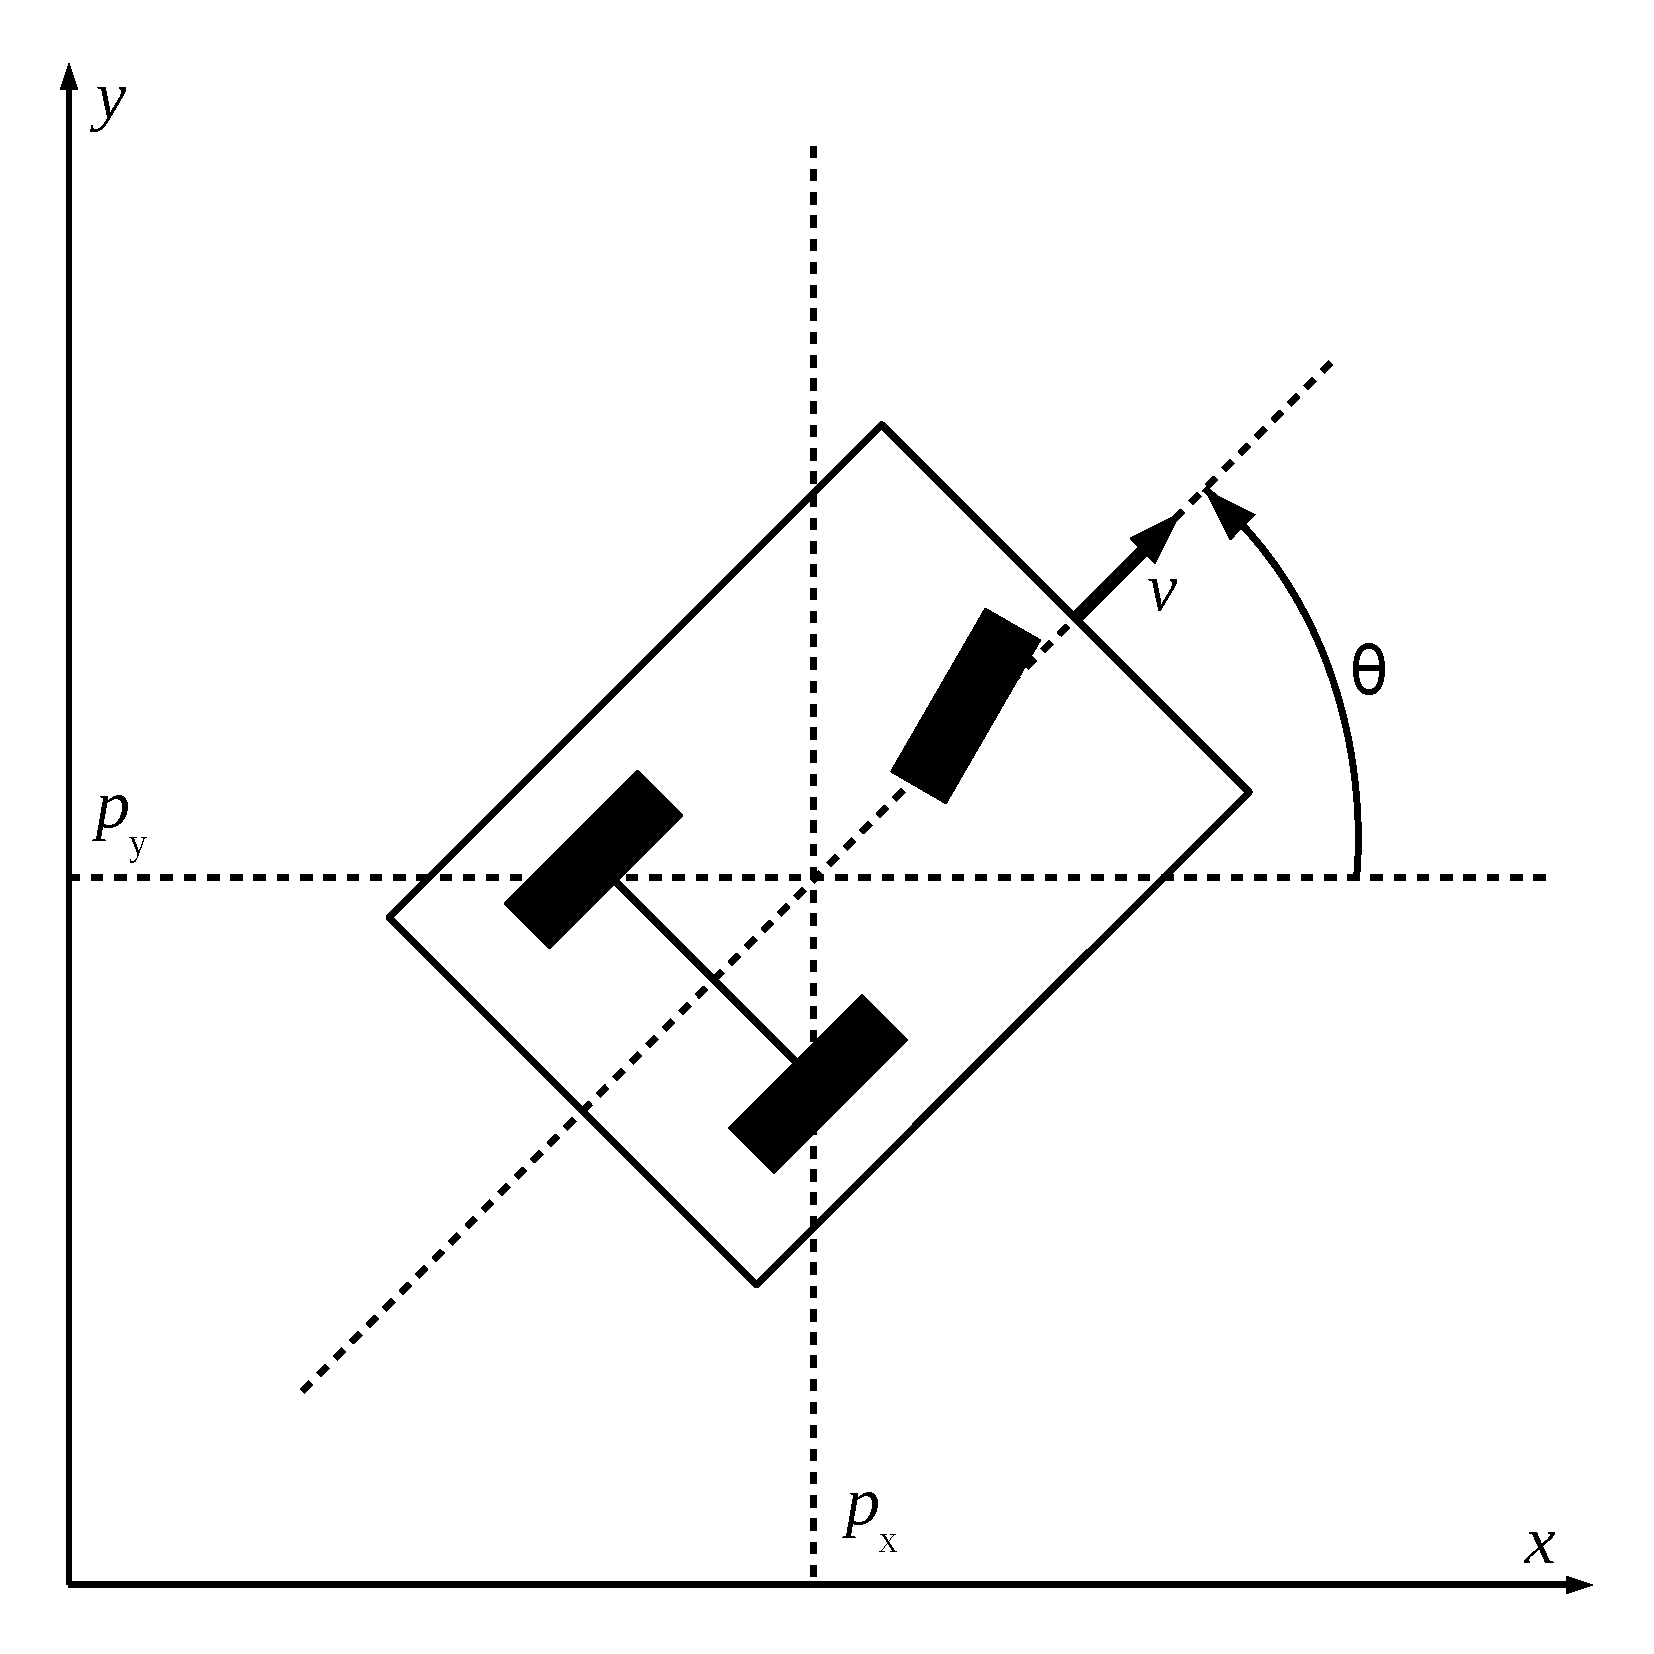
\includegraphics[width=0.4\textwidth]{Imagens/Nonholomonic-robot.pdf}
	\caption[Nonholomonic robot system representation]{Nonholomonic robot system representation. The system states $p_\textrm{x}$, $p_\textrm{y}$, $v$ and $\theta$ are highlighted.}
	\label{fig:robot}
\end{figure} 

The system described by~\ref{eq:sistema} is discretized by a fourth order Runge-Kutta method as described in Section~\ref{sec:discretization} and the state vector $x_i$ is given by $x_i \overset{\Delta}{=} [p_{\textrm{x},i}\ p_{\textrm{y},i}\ \theta_i\ v_i]^T$.

The observation model $y(t_k) \in \mathbb{R}^2$

\begin{equation}
y(t_k) = 
\begin{bmatrix}
p_\textrm{x}(t_k) \\
p_\textrm{y}(t_k)
\end{bmatrix}+v(t_k), \\
\end{equation}

\noindent
is given by the position coordinates and $\rho(v(t_k)) = \mathcal{N} (0,R_{t_k})$ is the observation noise, with zero mean and covariance $R_{t_k}$. When time-stamp is not available, the observation vector is approximated by $\tilde{y}_i \approx y(t_k)$, where $i$ is the index of the next time instant, multiple of $T$.

Input vector $u_i = [\omega_i\ a_i]^T$ is measured by a girometer and accelerometer, respectively. We assume that 

\begin{equation}\label{eq:entrada}
u_i = \tilde{u}_i - w_i,
\end{equation}

\noindent
where $\tilde{u}$ represent the sensors' measured values and $\rho(w) = \mathcal{N} (0, Q_i)$ is the corresponded noise, of zero mean and covariance $Q_i$. 

We simulate 60 seconds of robot movement, considering a step size of $\delta t_{\textrm{sim}} = 10^{-4}$. Irregular sampling time intervals $h_k$ are simulated by the exponential probability distribution function from Matlab\texttrademark \ and approximated to the nearest discrete time instant, from the 600,000 available samples. Input signals were generated arbitrarily according to Figure~\ref{fig:entrada}. Figure~\ref{fig:exukf} shows robot trajectory on $xy$-plane for the given input signals, leaving from point $(0,0)$, as well as a realization of noisy and aperiodic measurements with signal-to-noise ratio of SNR\textsubscript{y} $= 30$ dB and $\lambda=3.33$ Hz as red dots and the hatched blue line represents UKF estimation, considering time-stamp, $\alpha=5$ and SNR\textsubscript{u} $= 10$ dB. 


\begin{figure}[!htb]
	\centering
	\subfigure{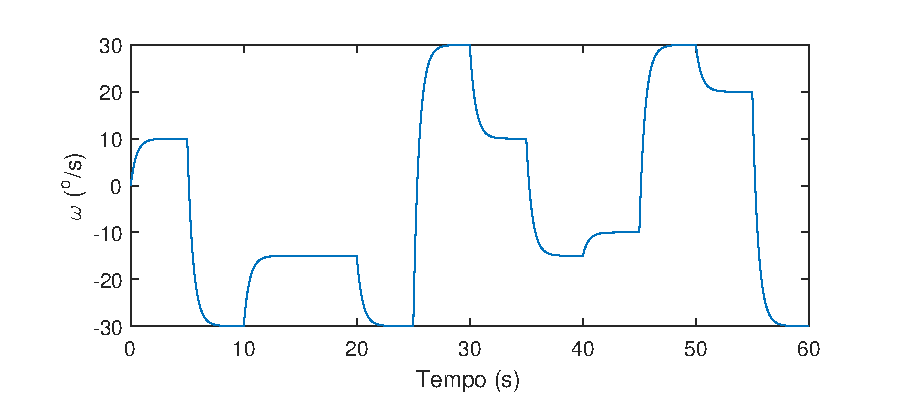
\includegraphics[width=0.8\textwidth]{Imagens/entradas1.eps}} \\
	\subfigure{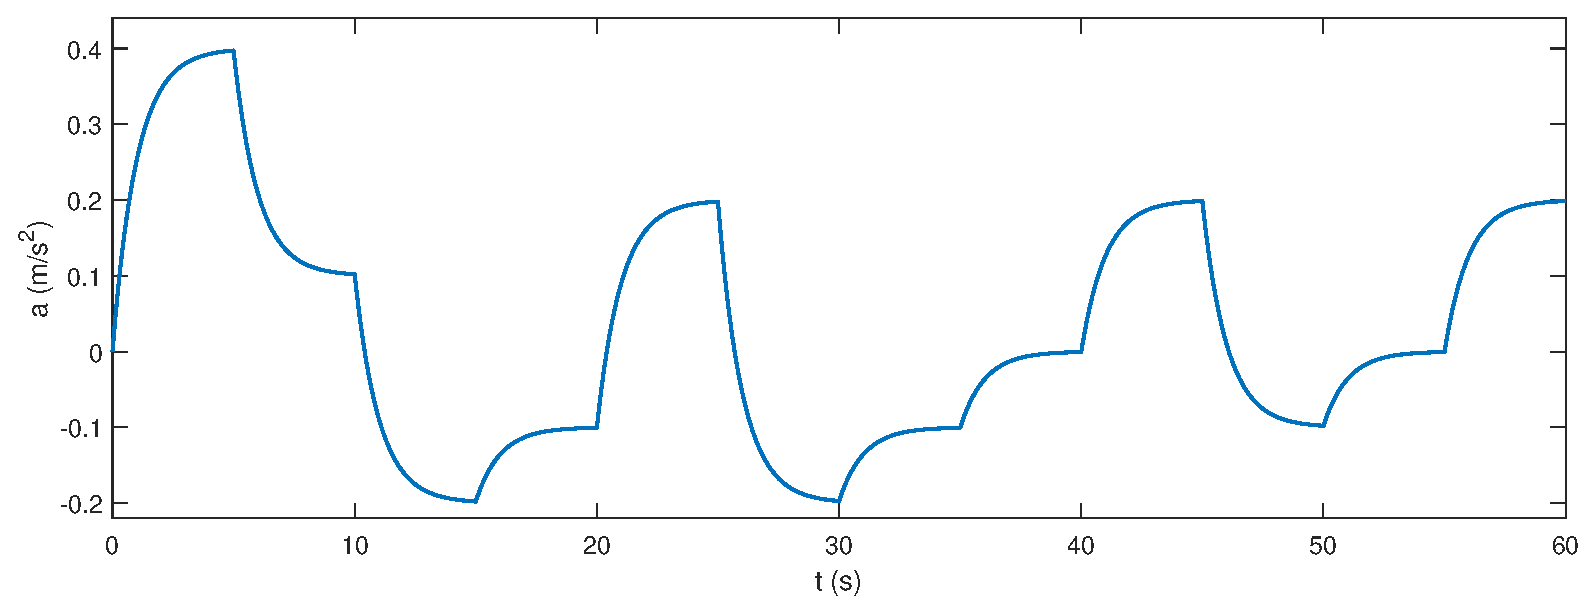
\includegraphics[width=0.8\textwidth]{Imagens/entradas2.eps}}  
	\caption[Simulation input signals]{Simulation input signals. (a) shows temporal sequence of angular velocity $\omega$ and (b) shows linear acceleration $a$.}
	\label{fig:entrada}
\end{figure}



\begin{figure}[!htb]
	\centering
	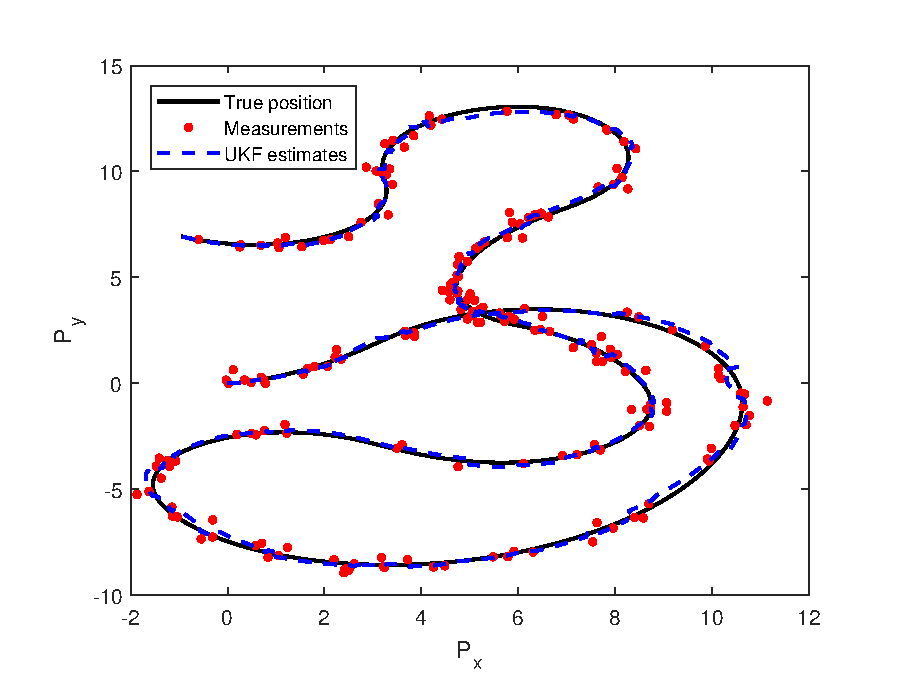
\includegraphics[width=0.8\textwidth]{Imagens/exemplo_03_30db_desloc.eps}
	\caption[True position, noisy measurements and UKF estimates]{True position, noisy measurements and UKF estimates considering time-stamp, for a measurement noise of SNR\textsubscript{y} $= 30$ dB, $\lambda=0.3$ s and $\alpha=5$.}
	\label{fig:exukf}
\end{figure} 

To analyze the effect of assimilating data at incorrect time instants in the estimation algorithm, we use the performance index $J$

\begin{equation}\label{eq:inddesemp}
J = \frac{ \sum_{i=1}^N \sqrt{(\hat{p}_{\textrm{x},i}-p_{\textrm{x},i})^2+(\hat{p}_{\textrm{y},i}-p_{\textrm{y},i})^2}}{N}
\end{equation}

\noindent
where $\hat{p}_{\textrm{x},i}$ and $\hat{p}_{\textrm{y},i}$ are filter position estimates produced at a regular interval $T$, $\hat{p}_{\textrm{x},i}$ and $\hat{p}_{\textrm{y},i}$ the true coordinates of the robot at the same time instants and $N$ the total number of estimates. This index represents the average estimator position error in $xy$-plane, similar to RMSE.

Figure~\ref{fig:realizacaoJ} shows a timespan from 0 to 1.3 seconds of a $J$ realization, considering $\lambda=0.5$, $\alpha=5$, SNR\textsubscript{y} $=60dB$ dB and SNR\textsubscript{u} $=20$ dB, for the UKF considering and not considering time-stamp. Black dots represent the regular time instants $kT$ whereas the asterisks on x-axis match the exact measurement instants $t_k$. As expected, before the first data assimilation steps, both performances are identical. Since the first measurement $t_1$ was taken almost at the same time as regular estimation time instant $4T$, both estimation performances maintain close to each other. That is because the approximation error due to $\tilde{y}_i \approx y(t_k)$ is irrelevant. At $t_2$ we can observe significant deviation from index $J$ in benefit of the algorithm considering time-stamp, since it performs data assimilation at the exact time measurement was taken. The same effect can be noted at $t_4$, after 1 second of simulation, when there is a significant different between time the measurement was taken and the next regular estimation instant.


\begin{figure}[!htb]
	\centering
	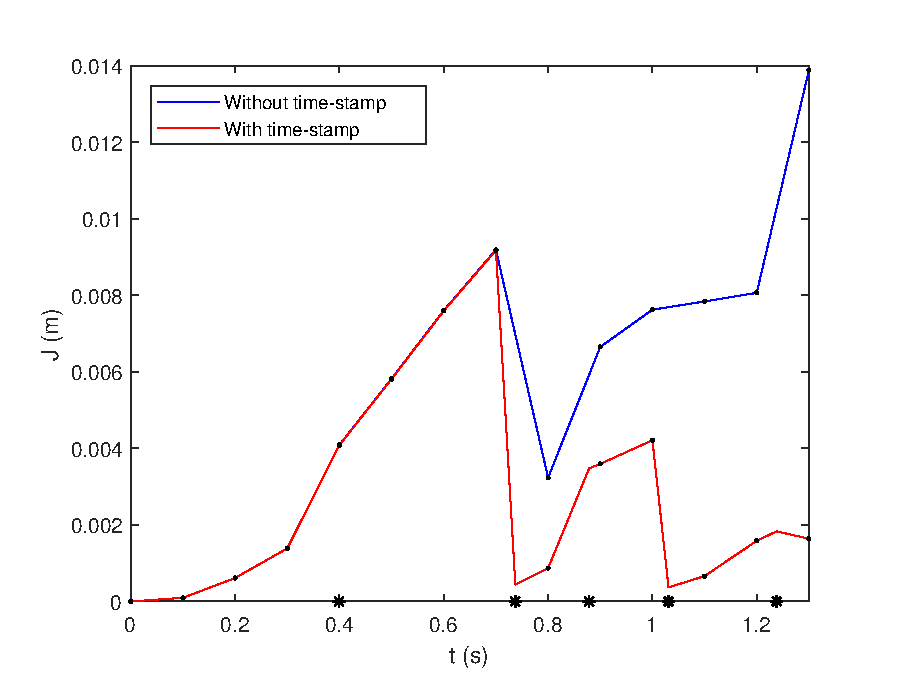
\includegraphics[width=0.8\textwidth]{Imagens/J_umarealizacao.eps}
	\caption[Performance index temporal cut for one realization]{Temporal cut from 0 to 1.3 seconds, for a realization of $J$ of both estimators, with and without time-stamp. Asterisks on $x$ axis match the measurement sampling instants $t_k$. Black dots represent the regular estimation instants, same as input regular sampling instants.}
	\label{fig:realizacaoJ}
\end{figure} 

%\begin{figure}[!htb]
%	\centering
%	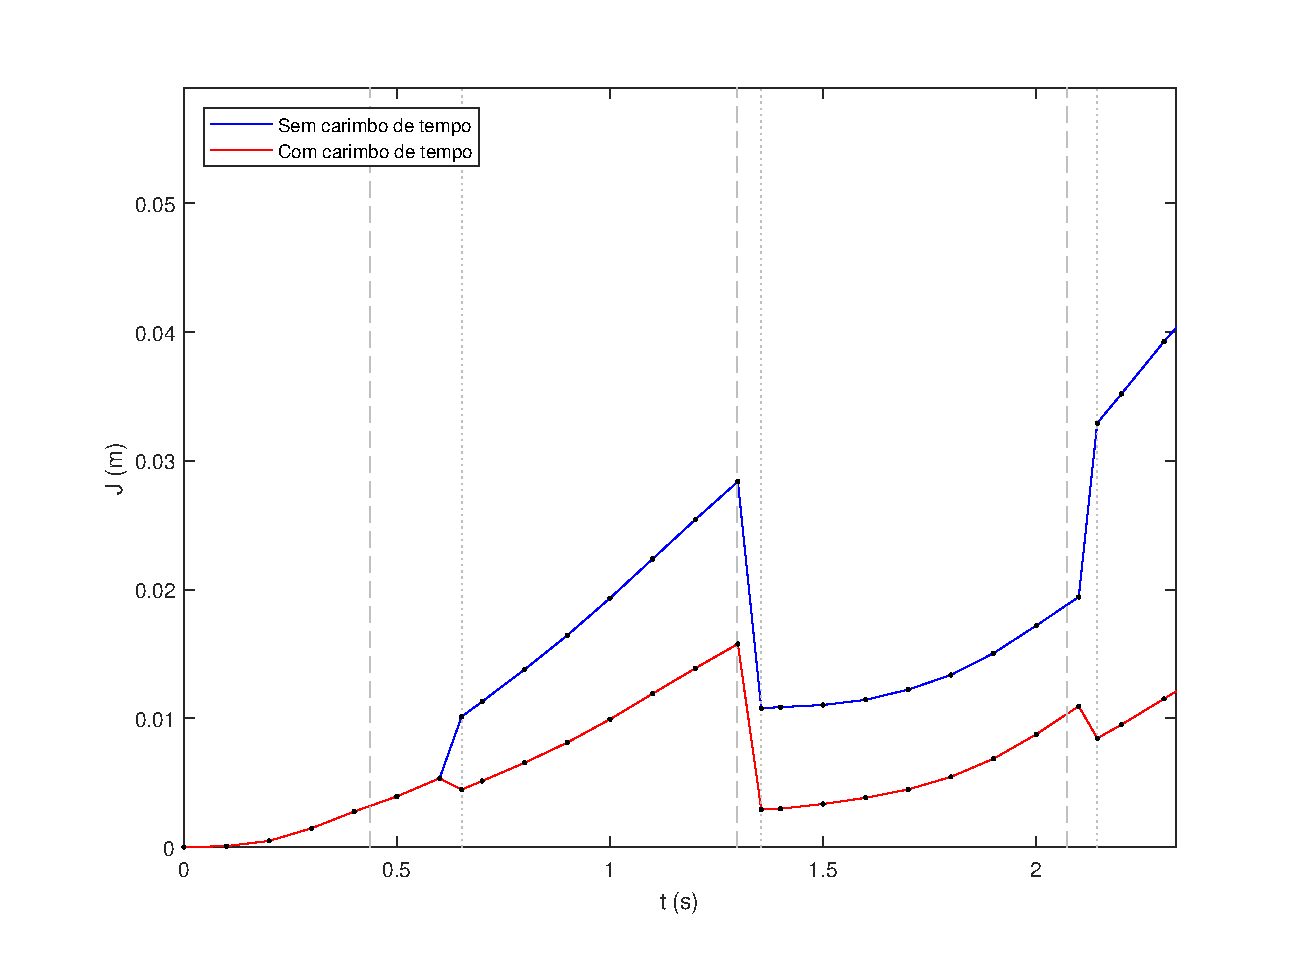
\includegraphics[width=0.8\textwidth]{Imagens/J_umarealizacao-timedelay.eps}
%%%	\caption[entrada]{Recorte temporal de 1 a 1.3 segundo, do �ndice J de uma realiza��o dos dois estimadores, com e sem carimbo de tempo. Os asteriscos no eixo $x$ representam os instantes de amostragem das observa��es $t_k$. Os pontos pretos apresentados nas linhas representam os instantes de tempo regulares de amostragem da entrada}
%	\label{fig:realizacaoJ2}
%\end{figure} 



%\setlength{\abovedisplayskip}{0.5pt}
%
%\begin{equation}\label{eq:sistema}
%\begin{split}
%\dot{\delta_e} & = -\tau^{-1},\\
%\dot{W} & = Z_{de}\delta_e + Z_wW + S_0q,\\
%\dot{q}  & = S_1 \delta_e + S_2 W + S_3q,\\
%\end{split}
%\end{equation}
%\noindent

\subsection{Measurement Signal-to-Noise Ratio Variation}\label{sec:ruido-robo}

In this subsection we compare the estimation performance impact of considering time-stamp in the algorithm, by varying the measurement noise level. The signal-to-noise ratio for the input sensors and the measurement average time interval are held constant, SNR\textsubscript{u} $= 20$ dB and $\lambda = 0.1$ s.

We considered an observation signal-to-noise variation of SNR\textsubscript{y} = $\infty$,  $80$, $60$, $40$, $20$, $10$ dB. That is, initially the system was simulated considering no measurement noise and then it was gradually increased. For each noise scenario, we ran 100 realizations of the random variables for each algorithm and Figure~\ref{fig:noise} shows the results. Solid lines represent the average values for $J$ and the dashed lines are the 95\% confidence interval.

\begin{figure}[!htb]
	\centering
	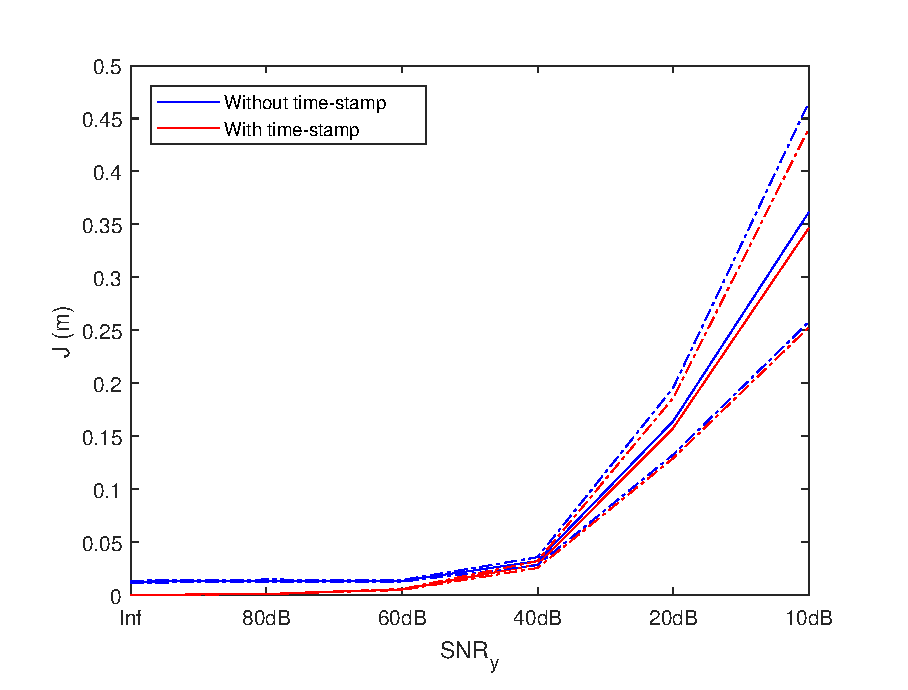
\includegraphics[width=0.8\textwidth]{Imagens/noise.eps}
	\caption[Performance index $J$ variation, as a function of measurement noise]{Performance index $J$ variation, as a function of measurement noise for both UKF algorithms considering and not considering time-stamp}
	\label{fig:noise}
\end{figure} 

Only for small noise levels, that is high SNR values, there are statistically significant difference between performances, in favor of knowing the exact time-instants. When $SNR_{y}$ is infinite or as high as $80$ dB, the performance index $J$ accuracy difference is approximately $1.25$ and $1.26$ cm, respectively. For SNR values lower than $40$ dB, however, it is not possible to distinguish among performances of both estimators.


\subsection{Average Sampling Rate Variation}\label{sec:lambda-robot}

We now consider the variation of the average time interval that observations are taken, according to $\lambda =$ $0.1$, $0.2$, $0.3$, $0.4$, $0.5$, $0.6$ s, maintaining the other parameters constant, namely the noise level of inputs and observations, SNR\textsubscript{u} $= 20$ dB and SNR\textsubscript{y} $= 40$ dB, respectively. We carried out 100 realizations for each $\lambda$ and for each algorithm and Figure~\ref{fig:samp} presents the results. Again, the solid lines are the average values of $J$ and the 95\% confidence interval is between the dashed lines.

\begin{figure}[!htb]
	\centering
	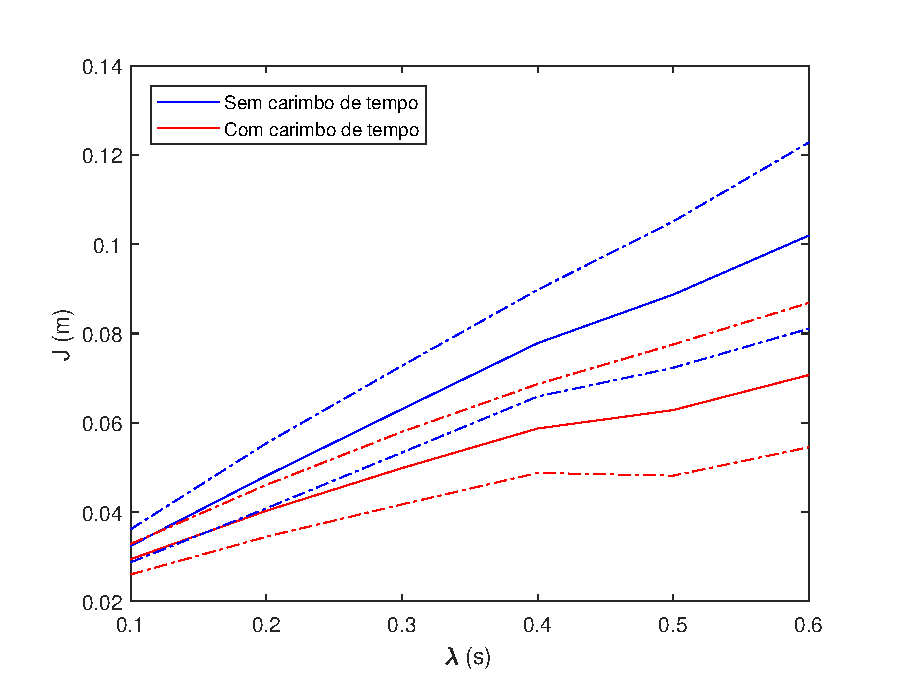
\includegraphics[width=0.8\textwidth]{Imagens/samp.eps}
	\caption[Performance index $J$ variation, as a function of $\lambda$]{Performance index $J$ variation, as a function of measurement noise both UKF algorithms considering and not considering time-stamp}
	\label{fig:samp}
\end{figure}

Results show that performance degradation is more significant for more spaced time intervals, if dynamics and other parameters are kept fixed. For higher  $\frac{1}{\lambda}$ rates, there are no statistical differences in performance. As average time interval grows, degradation increases and it starts to be apparent, reaching mean differences of $3.1$ cm for a $\lambda = 1.667$ Hz. One possible explanation derives from the fact if average sampling rate is considerably higher than system dynamics speed, time instant $t_k$ approximations errors are reduced. In such cases, sensor noise might end up being much more relevant than the error tunned by assimilating data at incorrect instants.

\subsection{Regular and Average Irregular Time Interval Relation Variation}\label{sec:alpha-robot}

We also analyze the performance impact of varying the parameter $\alpha$, which is the relation between regular input time interval $T$ and average measurements time interval $\lambda$. The simulated values were $\alpha = 10$, $5$, $2$, $1$. That means we start with higher frequency values for input sampling in comparison to measurement sampling and this values is gradually decreased. Other parameters were maintained constant SNR\textsubscript{u} $= 20$ dB and SNR\textsubscript{y} $= 40$ dB.

The same way we did for the other scenarios, 100 realizations were simulated and Figure~\ref{fig:dtudty} presents the results. Solid lines are the average values for $J$ and dashed lines represent the 95\% confidence interval.

\begin{figure}[!htb]
	\centering
	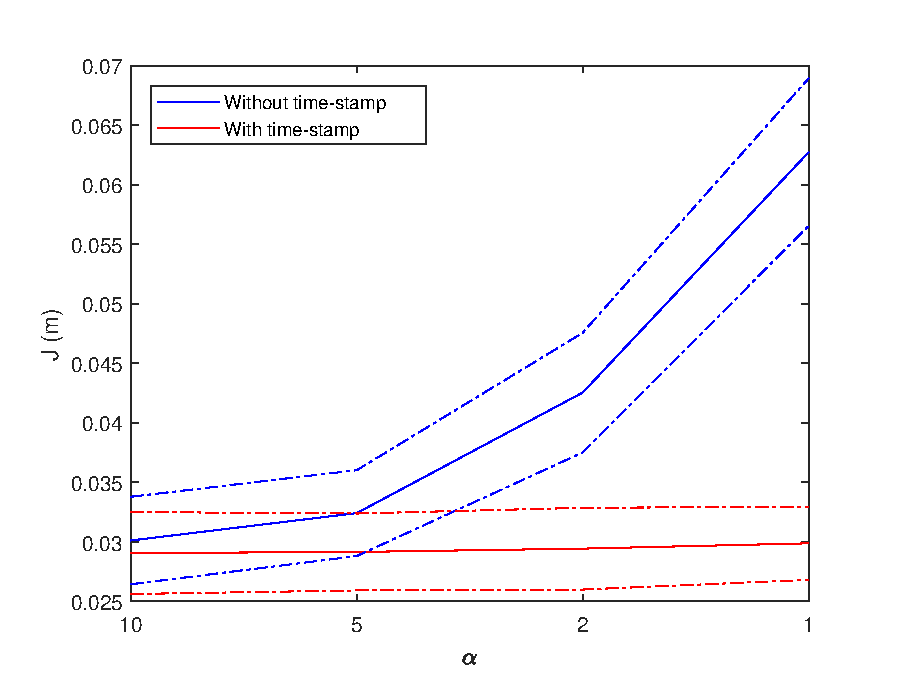
\includegraphics[width=0.8\textwidth]{Imagens/dtudty.eps}
	\caption[Performance index $J$ variation, as a function of $\alpha$]{Performance index $J$ variation, as a function of $\lambda$ for both UKF algorithms considering and not considering time-stamp}
	\label{fig:dtudty}
\end{figure}

The same way as it happened for the linear system, results suggest that when exact time instants $t_k$ are available, variations of $\alpha$ do not impact estimation performance. On the other hand, when time-stamp is not considering in the estimation process, the relation between regular estimation and average measurement time intervals plays an important role in estimates accuracy. The higher is the regular estimation rate in comparison to measurement rate, smaller is the degradation. In fact, for $\alpha$ values of 10 and 5, performances are statistically indistinguishable. When rates are the same, position estimate error doubled for the algorithm that does not consider time stamp. Such phenomenon can be explained by the fact that higher $\alpha$ values lead to smaller time steps used in the process model discretization in comparison to the measurement time intervals. Thus, approximation error originated from $\tilde{y}(i) \approx y(t_k)$ is reduced.


%\subsection{Average Time Delay}\label{sec:dt-robot}
%
%\todo[inline,caption={Falta variar o atraso nas medi��es}]{Ainda ter� uma se��o com a varia��o do time-delay e seu impacto no desempenho}


\clearpage
